\documentclass[../RASD.tex]{subfiles}
\graphicspath{{\subfix{../assets}}}

%From specific requirements
\usepackage{enumitem}
\usepackage{array}
\usepackage{amsmath}
\usepackage{float}
\usepackage{geometry}
\usepackage{color, xcolor}

\begin{document}
    \definecolor{ReqListRow1}{rgb}{0.8, 0.8, 0.8}
    \definecolor{ReqListCell2}{rgb}{0.863, 0.922, 0.967}
    \definecolor{ReqMappingRow1}{rgb}{0.8, 0.8, 0.8}
    \definecolor{ReqMappingCell2}{rgb}{0.863, 0.922, 0.967}
    \definecolor{ReqMappingCell3}{rgb}{1, 0.898, 0.831}
    \definecolor{UCMappingFirstRow}{HTML}{CCCCCC}
    \definecolor{UCMappingFirstColumn}{HTML}{D9E4DA}
    \definecolor{UCMappingSecondColumn}{HTML}{FFFFFF}

    \newlist{rlist}{enumerate}{1}
    \setlist[rlist,1]{label=\textbf{R\arabic*}:}

    \newcounter{rown}
    \setcounter{rown}{1}

    \newcommand{\rowIndex}{\arabic{rown}\stepcounter{rown}}
    \subsection{External Interface Requirements}

        \subsubsection{User Interfaces}
            CodeKataBattle's user interface will be used by both students and educators, so it should be easy to navigate and allow the use of all its functionalities to as many users as possible, regardless of the extent of their technical background. Therefore the interface has to be easy to use, intuitive and user-friendly on any kind of device.

        \subsubsection{Hardware Interfaces}
            The system revolves around the exchange of information and code solutions between the users and the system itself, so it doesn't require any specific external hardware interface to operate, it just needs to be securely reachable from the highest possible amount of people around the world
      
        \subsubsection{Software Interfaces}
            The system requires the presence of some external software interfaces in order to correctly operate:\\
            First of all, it requires some kind of repository service, to which educators will upload their code kata and which students will fork, in order to implement it with their code. Then each group of students will set up an automated procedure to inform CodeKataBattle of each new solution they will deliver through this system\\
            Once a new solution will be delivered by each group the application needs to have an automated evaluation system with which to automatically evaluate the functional aspects (measured in terms of number of test cases that are passed out of all the test cases, the higher the better), the timeliness (measured in terms of time passed between the registration deadline and the last commit performed by the group which made the delivery, the lower the better) and the quality level (extracted using static analysis tools that will consider aspects such as security, reliability, and maintainability of the code, the higher the better) of the sources obtained from the repository.\\
            Finally, for many important events that will take place while using the application (for example the creation of a tournament or the early closure of a battle), the system will use some kind of notification system to inform the user that such events have taken place (this system can be emails, windows notifications, smartphone notifications, sms or others), those notifications should also often (if possible) have some sort of way to quickly go from the notification itself straight to the application point of interest where that specific action is requested to the user (for example by clicking on the notification itself or by clicking/copying a possible direct link contained in the notification)
            \restoregeometry

            Regarding the user instead, to access the system itself no particular software is required, but such software is necessary to develop the solution to be delivered. In order to do that theoretically just a text editor would be enough, but the use of an Integrated Development Environment (IDE) instead is strongly suggested, since it would make the development of such solution much easier and allow a more straightforward quick testing before the delivery

        \subsubsection{Communication Interfaces}
            As already mentioned, the system revolves around the exchange of information and code solutions between the users and the system itself, so the system needs to be securely reachable from the highest possible amount of people around the world, to assure that communications will allways be enrypted using TLS 1.3 by the usage of the HTTPS protocol for each communication

    \newpage
    \subsection{Functional Requirements}
    \subsubsection{List of requirements}
    \underline{Sign up and profile requirements:}
        \begin{table}[ht]
            \begin{center}
                \begin{tabular}{|m{2em}|m{35em}|}
                \hline
                \rowcolor{ReqListRow1}
                \textbf{ID} & \textbf{Requirement}\\
                \hline
                \cellcolor{ReqListCell2}
                \textbf{R\rowIndex} & The system must allow the registration of new users using their e-mail\\
                \hline
                \cellcolor{ReqListCell2}
                \textbf{R\rowIndex} & The system must notify a user about his/her successful registration\\
                \hline
                \cellcolor{ReqListCell2}
                \textbf{R\rowIndex} & The system must allow registered users to log-in using their e-mail.\\
                \hline
                \cellcolor{ReqListCell2}
                \textbf{R\rowIndex} & The system must allow logged-in users to use the application.\\
                \hline
                \cellcolor{ReqListCell2}
                \textbf{R\rowIndex} & The system must respect the GDPR\\
                \hline
                \cellcolor{ReqListCell2}
                \textbf{R\rowIndex} & The system must allow a user to set a nickname for his/her profile\\
                \hline
                \cellcolor{ReqListCell2}
                \textbf{R\rowIndex} & The system must allow a user to set a phone number for his/her profile\\
                \hline
                \end{tabular}
            \end{center}
        \end{table}\newpage
    \underline{Tournaments and battles creation requirements:}
        \begin{table}[h!]
            \begin{center}
                \begin{tabular}{|m{2em}|m{35em}|}
                \hline
                \rowcolor{ReqListRow1}
                \textbf{ID} & \textbf{Requirement}\\
                \hline
                \cellcolor{ReqListCell2}
                \textbf{R\rowIndex} & The system must allow an educator to create a tournament if another tournament with the same name doesn't already exist\\
                \hline
                \cellcolor{ReqListCell2}
                \textbf{R\rowIndex} & The system must reject an educator request to create a tournament if another tournament with the same name already exist\\
                \hline
                \cellcolor{ReqListCell2}
                \textbf{R\rowIndex} & The system must allow the owner of a tournament to invite other educators to manage it\\
                \hline
                \cellcolor{ReqListCell2}
                \textbf{R\rowIndex} & The system must notify an educator when he/she is invited to manage a tournament\\
                \hline
                \cellcolor{ReqListCell2}
                \textbf{R\rowIndex} & The system must allow an educator to accept the invitation of another educator to manage a tournament\\
                \hline
                \cellcolor{ReqListCell2}
                \textbf{R\rowIndex} & The system must allow an educator to set a registration deadline when creating a tournament\\
                \hline
                \cellcolor{ReqListCell2}
                \textbf{R\rowIndex} & The system must allow to set a minimum number of students for each group when creating a new battle\\
                \hline
                \cellcolor{ReqListCell2}
                \textbf{R\rowIndex} & The system must allow to set the maximum number of students for each group when creating a new battle\\
                \hline
                \cellcolor{ReqListCell2}
                \textbf{R\rowIndex} & The system must allow to set a registration deadline when creating a new battle\\
                \hline
                \cellcolor{ReqListCell2}
                \textbf{R\rowIndex} & The system must allow to set a final submission deadline when creating a new battle\\
                \hline
                \cellcolor{ReqListCell2}
                \textbf{R\rowIndex} & The system must allow an educator to choose while creating a new battle which aspects of the quality level of the sources will be automatically evaluated \\
                \hline
                \cellcolor{ReqListCell2}
                \textbf{R\rowIndex} & The system must allow an educator to choose while creating a new battle whether a manual evaluation will be needed after the automated ones\\
                \hline
                \cellcolor{ReqListCell2}
                \textbf{R\rowIndex} & The system must be able to receive a new code kata from an educator when he/she is creating a battle\\
                \hline
                \cellcolor{ReqListCell2}
                \textbf{R\rowIndex} & The system must allow the educators managing a tournament to create new battles in the context of such tournament\\
                \hline
                \cellcolor{ReqListCell2}
                \textbf{R\rowIndex} & The system must notify all users of the platform when a new tournament is created\\
                \hline
                \cellcolor{ReqListCell2}
                \textbf{R\rowIndex} & The system must notify all students subscribed to that tournament when a new battle of such tournament starts\\
                \hline
                \end{tabular}
            \end{center}
        \end{table}\newpage
    \underline{Ongoing tournament requirements:}
    \begin{table}[ht]
        \begin{center}
            \begin{tabular}{|m{2em}|m{35em}|}
            \hline
            \rowcolor{ReqListRow1}
            \textbf{ID} & \textbf{Requirement}\\
            \hline
            \cellcolor{ReqListCell2}
            \textbf{R\rowIndex} & The system must allow users to subscribe to a tournament\\
            \hline
            \cellcolor{ReqListCell2}
            \textbf{R\rowIndex} & The system must allow students to create groups in the context of a battle\\
            \hline
            \cellcolor{ReqListCell2}
            \textbf{R\rowIndex} & The system must allow a student to invite another to his/her own group, if such student is enrolled into the corresponding battle\\
            \hline
            \cellcolor{ReqListCell2}
            \textbf{R\rowIndex} & The system must reject a student request to invite another student to his/her own group, if such student is not enrolled into the corresponding battle\\
            \hline
            \cellcolor{ReqListCell2}
            \textbf{R\rowIndex} & The system must notify a student when he/she is invited to a group\\
            \hline
            \cellcolor{ReqListCell2}
            \textbf{R\rowIndex} & The system must allow a student to join an existing group if invited\\
            \hline
            \cellcolor{ReqListCell2}
            \textbf{R\rowIndex} & The system must allow groups to join a newly created battle if they respect that battle's constraints\\
            \hline
            \cellcolor{ReqListCell2}
            \textbf{R\rowIndex} & The system must allow all students enrolled into a battle, to access its code kata\\
            \hline
            \cellcolor{ReqListCell2}
            \textbf{R\rowIndex} & The system must allow a group to submit his/their solution\\
            \hline
            \cellcolor{ReqListCell2}
            \textbf{R\rowIndex} & The system must update a group battle score after each new solution is delivered\\
            \hline
            \cellcolor{ReqListCell2}
            \textbf{R\rowIndex} & The system must show to each group his/their rank in the current battle\\
            \hline
            \cellcolor{ReqListCell2}
            \textbf{R\rowIndex} & The system must show to each group his/their current battle score\\
            \hline
            \end{tabular}
        \end{center}
    \end{table}\newpage
    \underline{Tournaments and battles concluding requirements:}
    \begin{table}[h!]
        \begin{center}
            \begin{tabular}{|m{2em}|m{35em}|}
            \hline
            \rowcolor{ReqListRow1}
            \textbf{ID} & \textbf{Requirement}\\
            \hline
            \cellcolor{ReqListCell2}
            \textbf{R\rowIndex} & The system must notify all students subscribed to a tournament when the consolidation phase of a battle of such tournament has ended\\
            \hline
            \cellcolor{ReqListCell2}
            \textbf{R\rowIndex} & The system must be able to evaluate functional aspects of a group's delivery\\
            \hline
            \cellcolor{ReqListCell2}
            \textbf{R\rowIndex} & The system must be able to evaluate the timeliness of a group's delivery\\
            \hline
            \cellcolor{ReqListCell2}
            \textbf{R\rowIndex} & The system must be able to evaluate the quality level of the sources of a group's delivery\\
            \hline
            \cellcolor{ReqListCell2}
            \textbf{R\rowIndex} & The system must show the results of its automated analysis to the educators managing the tournament\\
            \hline
            \cellcolor{ReqListCell2}
            \textbf{R\rowIndex} & The system must allow an educator to see the solution provided by each group\\
            \hline
            \cellcolor{ReqListCell2}
            \textbf{R\rowIndex} & The system must allow an educator to manually mark a solution in the consolidation phase, if this was set up in the initial configuration of the battle\\
            \hline
            \cellcolor{ReqListCell2}
            \textbf{R\rowIndex} & The system must update the tournament score of each student participating into that tournament after the consolidation phase has ended\\
            \hline
            \cellcolor{ReqListCell2}
            \textbf{R\rowIndex} & The system must allow a student to see his/her rank in a certain tournament\\
            \hline
            \cellcolor{ReqListCell2}
            \textbf{R\rowIndex} & The system must allow a student to see his/her tournament score\\
            \hline
            \cellcolor{ReqListCell2}
            \textbf{R\rowIndex} & The system must allow all users to see the list of ongoing tournaments\\
            \hline
            \cellcolor{ReqListCell2}
            \textbf{R\rowIndex} & The system must allow all users to see the current tournament score leaderboard for each ongoing tournament\\
            \hline
            \cellcolor{ReqListCell2}
            \textbf{R\rowIndex} & The system must allow an educator to close a battle before its expected conclusion\\
            \hline
            \cellcolor{ReqListCell2}
            \textbf{R\rowIndex} & The system must allow an educator to set up a message explaining his/her motivations when closing a battle ahead of time\\
            \hline
            \cellcolor{ReqListCell2}
            \textbf{R\rowIndex} & The system must notify all students subscribed to a tournament when a battle in such tournament is closed ahead of time\\
            \hline
            \cellcolor{ReqListCell2}
            \textbf{R\rowIndex} & The system must show the educator's motivation message when notifying students about the early closure of a battle\\
            \hline
            \cellcolor{ReqListCell2}
            \textbf{R\rowIndex} & The system must allow an educator to close a tournament, if there is not an ongoing battle in such tournament\\
            \hline
            \cellcolor{ReqListCell2}
            \textbf{R\rowIndex} & The system must reject an educator request to close a tournament, if there is an ongoing battle in such tournament\\
            \hline
            \cellcolor{ReqListCell2}
            \textbf{R\rowIndex} & The system must notify all students subscribed to a tournament when such tournament is closed\\
            \hline
            \end{tabular}
        \end{center}
    \end{table}\newpage
    \subsubsection{Mapping}
    \underline{User goals}
        \begin{table}[ht]
            \begin{center}
                \begin{tabular}{|m{2em}|m{30em}|}
                \hline
                \rowcolor{ReqMappingRow1}
                \textbf{G1} & \textbf{Have his/her own profile on the application}\\
                \hline
                \cellcolor{ReqMappingCell2}
                \textbf{R1} & The system must allow the registration of new users using their e-mail\\
                \hline
                \cellcolor{ReqMappingCell2}
                \textbf{R2} & The system must notify a user about his/her successful registration\\
                \hline
                \cellcolor{ReqMappingCell2}
                \textbf{R3} & The system must allow registered users to log-in using their e-mail.\\
                \hline
                \cellcolor{ReqMappingCell2}
                \textbf{R4} & The system must allow logged-in users to use the application.\\
                \hline
                \cellcolor{ReqMappingCell2}
                \textbf{R5} & The system must respect the GDPR\\
                \hline
                \cellcolor{ReqMappingCell2}
                \textbf{R6} & The system must allow a user to set a nickname for his/her profile\\
                \hline
                \cellcolor{ReqMappingCell2}
                \textbf{R7} & The system must allow a user to set a phone number for his/her profile\\
                \hline
                \cellcolor{ReqMappingCell3}
                \textbf{D1} & Users have internet access while using the application\\
                \hline
                \cellcolor{ReqMappingCell3}
                \textbf{D2} & Users have only one account\\
                \hline
                \end{tabular}
            \end{center}
        \end{table}\newpage
        \begin{table}[ht]
            \begin{center}
                \begin{tabular}{|m{2em}|m{30em}|}
                \hline
                \rowcolor{ReqMappingRow1}
                \textbf{G2} & \textbf{Participate in a coding tournament}\\
                \hline
                \cellcolor{ReqMappingCell2}
                \textbf{R3} & The system must allow registered users to log-in using their e-mail.\\
                \hline
                \cellcolor{ReqMappingCell2}
                \textbf{R4} & The system must allow logged-in users to use the application.\\
                \hline
                \cellcolor{ReqMappingCell2}
                \textbf{R5} & The system must respect the GDPR\\
                \hline
                \cellcolor{ReqMappingCell2}
                \textbf{R8} & The system must allow an educator to create a tournament if another tournament with the same name doesn't already exist\\
                \hline
                \cellcolor{ReqMappingCell2}
                \textbf{R22} & The system must notify all users of the platform when a new tournament is created\\
                \hline
                \cellcolor{ReqMappingCell2}
                \textbf{R24} & The system must allow users to subscribe to a tournament\\
                \hline
                \cellcolor{ReqMappingCell2}
                \textbf{R31} & The system must allow all students enrolled into a battle, to access its code kata\\
                \hline
                \cellcolor{ReqMappingCell2}
                \textbf{R32} & The system must allow a group to submit his/their solution\\
                \hline
                \cellcolor{ReqMappingCell2}
                \textbf{R46} & The system must allow all users to see the list of ongoing tournaments\\
                \hline
                \cellcolor{ReqMappingCell3}
                \textbf{D1} & Users have internet access while using the application\\
                \hline
                \cellcolor{ReqMappingCell3}
                \textbf{D2} & Users have only one account\\
                \hline
                \cellcolor{ReqMappingCell3}
                \textbf{D3} & Users device always send correct data to the application regarding its specifications\\
                \hline
                \cellcolor{ReqMappingCell3}
                \textbf{D4} & The repository service is reliable and works 99.9\% of the time\\
                \hline
                \cellcolor{ReqMappingCell3}
                \textbf{D5} & Users have the ability to interact and correctly use the repository platform\\
                \hline
                \cellcolor{ReqMappingCell3}
                \textbf{D6} & Users notification system is reliable and works 99.9\% of the time\\
                \hline
                \cellcolor{ReqMappingCell3}
                \textbf{D7} & Users won't block notifications coming from the application\\
                \hline
                \end{tabular}
            \end{center}
        \end{table}\newpage

        \begin{table}[h!]
            \begin{center}
                \begin{tabular}{|m{2em}|m{30em}|}
                \hline
                \rowcolor{ReqMappingRow1}
                \textbf{G3} & \textbf{Cooperate with colleagues}\\
                \hline
                \cellcolor{ReqMappingCell2}
                \textbf{R3} & The system must allow registered users to log-in using their e-mail.\\
                \hline
                \cellcolor{ReqMappingCell2}
                \textbf{R4} & The system must allow logged-in users to use the application.\\
                \hline
                \cellcolor{ReqMappingCell2}
                \textbf{R5} & The system must respect the GDPR\\
                \hline
                \cellcolor{ReqMappingCell2}
                \textbf{R25} & The system must allow students to create groups in the context of a battle\\
                \hline
                \cellcolor{ReqMappingCell2}
                \textbf{R26} & The system must allow a student to invite another to his/her own group, if such student is enrolled into the corresponding battle\\
                \hline
                \cellcolor{ReqMappingCell2}
                \textbf{R27} & The system must reject a student request to invite another student to his/her own group, if such student is not enrolled into the corresponding battle\\
                \hline
                \cellcolor{ReqMappingCell2}
                \textbf{R28} & The system must notify a student when he/she is invited to a group\\
                \hline
                \cellcolor{ReqMappingCell2}
                \textbf{R29} & The system must allow a student to join an existing group if invited\\
                \hline
                \cellcolor{ReqMappingCell2}
                \textbf{R30} & The system must allow groups to join a newly created battle if they respect that battle's constraints\\
                \hline
                \cellcolor{ReqMappingCell2}
                \textbf{R31} & The system must allow all students enrolled into a battle, to access its code kata\\
                \hline
                \cellcolor{ReqMappingCell2}
                \textbf{R32} & The system must allow a group to submit his/their solution\\
                \hline
                \cellcolor{ReqMappingCell2}
                \textbf{R33} & The system must update a group battle score after each new solution is delivered\\
                \hline
                \cellcolor{ReqMappingCell2}
                \textbf{R34} & The system must show to each group his/their rank in the current battle\\
                \hline
                \cellcolor{ReqMappingCell2}
                \textbf{R35} & The system must show to each group his/their current battle score\\
                \hline
                \cellcolor{ReqMappingCell3}
                \textbf{D1} & Users have internet access while using the application\\
                \hline
                \cellcolor{ReqMappingCell3}
                \textbf{D2} & Users have only one account\\
                \hline
                \cellcolor{ReqMappingCell3}
                \textbf{D3} & Users device always send correct data to the application regarding its specifications\\
                \hline
                \cellcolor{ReqMappingCell3}
                \textbf{D4} & The repository service is reliable and works 99.9\% of the time\\
                \hline
                \cellcolor{ReqMappingCell3}
                \textbf{D5} & Users have the ability to interact and correctly use the repository platform\\
                \hline
                \cellcolor{ReqMappingCell3}
                \textbf{D6} & Users notification system is reliable and works 99.9\% of the time\\
                \hline
                \cellcolor{ReqMappingCell3}
                \textbf{D7} & Users won't block notifications coming from the application\\
                \hline
                \cellcolor{ReqMappingCell3}
                \textbf{D9} & Users who are members of the same group will contribute equally to the delivery\\
                \hline
                \end{tabular}
            \end{center}
        \end{table}\newpage

        \begin{table}[ht]
            \begin{center}
                \begin{tabular}{|m{2em}|m{30em}|}
                \hline
                \rowcolor{ReqMappingRow1}
                \textbf{G4} & \textbf{Review their own performance score}\\
                \hline
                \cellcolor{ReqMappingCell2}
                \textbf{R3} & The system must allow registered users to log-in using their e-mail.\\
                \hline
                \cellcolor{ReqMappingCell2}
                \textbf{R4} & The system must allow logged-in users to use the application.\\
                \hline
                \cellcolor{ReqMappingCell2}
                \textbf{R5} & The system must respect the GDPR\\
                \hline
                \cellcolor{ReqMappingCell2}
                \textbf{R33} & The system must update a group battle score after each new solution is delivered\\
                \hline
                \cellcolor{ReqMappingCell2}
                \textbf{R34} & The system must show to each group his/their rank in the current battle\\
                \hline
                \cellcolor{ReqMappingCell2}
                \textbf{R35} & The system must show to each group his/their current battle score\\
                \hline
                \cellcolor{ReqMappingCell2}
                \textbf{R43} & The system must update the tournament score of each student participating into that tournament after the consolidation phase has ended\\
                \hline
                \cellcolor{ReqMappingCell2}
                \textbf{R44} & The system must allow a student to see his/her rank in a certain tournament\\
                \hline
                \cellcolor{ReqMappingCell2}
                \textbf{R45} & The system must allow a student to see his/her tournament score\\
                \hline
                \cellcolor{ReqMappingCell2}
                \textbf{R47} & The system must allow all users to see the current tournament score leaderboard for each ongoing tournament\\
                \hline
                \cellcolor{ReqMappingCell3}
                \textbf{D1} & Users have internet access while using the application\\
                \hline
                \cellcolor{ReqMappingCell3}
                \textbf{D3} & Users device always send correct data to the application regarding its specifications\\
                \hline
                \cellcolor{ReqMappingCell3}
                \textbf{D8} & The automated evaluation system is reliable and works 99.9\% of the time\\
                \hline
                \cellcolor{ReqMappingCell3}
                \textbf{D9} & Users who are members of the same group will contribute equally to the delivery\\
                \hline
                \cellcolor{ReqMappingCell3}
                \textbf{D10} & Users won't receive any external help from a person not in their group while competing in a battle\\
                \hline
                \cellcolor{ReqMappingCell3}
                \textbf{D11} & Educator's manual review of the delivery is unbiased\\
                \hline
                \end{tabular}
            \end{center}
        \end{table}\newpage

        \underline{Educator goals}
        \begin{table}[h!]
            \begin{center}
                \begin{tabular}{|m{2em}|m{30em}|}
                \hline
                \rowcolor{ReqMappingRow1}
                \textbf{G5} & \textbf{Organize coding tournaments}\\
                \hline
                \cellcolor{ReqMappingCell2}
                \textbf{R3} & The system must allow registered users to log-in using their e-mail.\\
                \hline
                \cellcolor{ReqMappingCell2}
                \textbf{R4} & The system must allow logged-in users to use the application.\\
                \hline
                \cellcolor{ReqMappingCell2}
                \textbf{R5} & The system must respect the GDPR\\
                \hline
                \cellcolor{ReqMappingCell2}
                \textbf{R8} & The system must allow an educator to create a tournament if another tournament with the same name doesn't already exist\\
                \hline
                \cellcolor{ReqMappingCell2}
                \textbf{R9} & The system must reject an educator request to create a tournament if another tournament with the same name already exist\\
                \hline
                \cellcolor{ReqMappingCell2}
                \textbf{R10} & The system must allow the owner of a tournament to invite other educators to manage it\\
                \hline
                \cellcolor{ReqMappingCell2}
                \textbf{R11} & The system must notify an educator when he/she is invited to manage a tournament\\
                \hline
                \cellcolor{ReqMappingCell2}
                \textbf{R12} & The system must allow an educator to accept the invitation of another educator to manage a tournament\\
                \hline
                \cellcolor{ReqMappingCell2}
                \textbf{R13} & The system must allow an educator to set a registration deadline when creating a tournament\\
                \hline
                \cellcolor{ReqMappingCell2}
                \textbf{R21} & The system must allow the educators managing a tournament to create new battles in the context of such tournament\\
                \hline
                \cellcolor{ReqMappingCell2}
                \textbf{R22} & The system must notify all users of the platform when a new tournament is created\\
                \hline
                \cellcolor{ReqMappingCell2}
                \textbf{R24} & The system must allow users to subscribe to a tournament\\
                \hline
                \cellcolor{ReqMappingCell2}
                \textbf{R52} & The system must allow an educator to close a tournament, if there is not an ongoing battle in such tournament\\
                \hline
                \cellcolor{ReqMappingCell2}
                \textbf{R53} & The system must reject an educator request to close a tournament, if there is an ongoing battle in such tournament\\
                \hline
                \cellcolor{ReqMappingCell2}
                \textbf{R54} & The system must notify all students subscribed to a tournament when such tournament is closed\\
                \hline
                \cellcolor{ReqMappingCell2}
                \textbf{D1} & Users have internet access while using the application\\
                \hline
                \cellcolor{ReqMappingCell3}
                \textbf{D3} & Users device always send correct data to the application regarding its specifications\\
                \hline
                \cellcolor{ReqMappingCell3}
                \textbf{D6} & Users notification system is reliable and works 99.9\% of the time\\
                \hline
                \cellcolor{ReqMappingCell3}
                \textbf{D7} & Users won't block notifications coming from the application\\
                \hline
                \end{tabular}
            \end{center}
        \end{table}\newpage

        \newgeometry{top=6em}
        \begin{table}[H]
            \begin{center}
                \begin{tabular}{|m{2em}|m{30em}|}
                \hline
                \rowcolor{ReqMappingRow1}
                \textbf{G6} & \textbf{Run coding battles in their tournaments}\\
                \hline
                \cellcolor{ReqMappingCell2}
                \textbf{R3} & The system must allow registered users to log-in using their e-mail.\\
                \hline
                \cellcolor{ReqMappingCell2}
                \textbf{R4} & The system must allow logged-in users to use the application.\\
                \hline
                \cellcolor{ReqMappingCell2}
                \textbf{R5} & The system must respect the GDPR\\
                \hline
                \cellcolor{ReqMappingCell2}
                \textbf{R8} & The system must allow an educator to create a tournament if another tournament with the same name doesn't already exist\\
                \hline
                \cellcolor{ReqMappingCell2}
                \textbf{R14} & The system must allow to set a minimum number of students for each group when creating a new battle\\
                \hline
                \cellcolor{ReqMappingCell2}
                \textbf{R15} & The system must allow to set the maximum number of students for each group when creating a new battle\\
                \hline
                \cellcolor{ReqMappingCell2}
                \textbf{R16} & The system must allow to set a registration deadline when creating a new battle\\
                \hline
                \cellcolor{ReqMappingCell2}
                \textbf{R17} & The system must allow to set a final submission deadline when creating a new battle\\
                \hline
                \cellcolor{ReqMappingCell2}
                \textbf{R18} & The system must allow an educator to choose while creating a new battle which aspects of the quality level of the sources will be automatically evaluated\\
                \hline
                \cellcolor{ReqMappingCell2}
                \textbf{R19} & The system must allow an educator to choose while creating a new battle whether a manual evaluation will be needed after the automated ones\\
                \hline
                \cellcolor{ReqMappingCell2}
                \textbf{R20} & The system must be able to receive a new code kata from an educator when he/she is creating a battle\\
                \hline
                \cellcolor{ReqMappingCell2}
                \textbf{R21} & The system must allow the educators managing a tournament to create new battles in the context of such tournament\\
                \hline
                \cellcolor{ReqMappingCell2}
                \textbf{R23} & The system must notify all students subscribed to that tournament when a new battle of such tournament starts\\
                \hline
                \cellcolor{ReqMappingCell2}
                \textbf{R30} & The system must allow groups to join a newly created battle if they respect that battle's constraints\\
                \hline
                \cellcolor{ReqMappingCell2}
                \textbf{R31} & The system must allow all students enrolled into a battle, to access its code kata\\
                \hline
                \cellcolor{ReqMappingCell2}
                \textbf{R32} & The system must allow a group to submit his/their solution\\
                \hline
                \cellcolor{ReqMappingCell3}
                \textbf{D1} & Users have internet access while using the application\\
                \hline
                \cellcolor{ReqMappingCell3}
                \textbf{D2} & Users have only one account\\
                \hline
                \cellcolor{ReqMappingCell3}
                \textbf{D3} & Users device always send correct data to the application regarding its specifications\\
                \hline
                \cellcolor{ReqMappingCell3}
                \textbf{D4} & The repository service is reliable and works 99.9\% of the time\\
                \hline
                \cellcolor{ReqMappingCell3}
                \textbf{D5} & Users have the ability to interact and correctly use the repository platform\\
                \hline
                \cellcolor{ReqMappingCell3}
                \textbf{D6} & Users notification system is reliable and works 99.9\% of the time\\
                \hline
                \cellcolor{ReqMappingCell3}
                \textbf{D7} & Users won't block notifications coming from the application\\
                \hline
                \end{tabular}
            \end{center}
        \end{table}\newpage

        \restoregeometry
        \begin{table}[ht]
            \begin{center}
                \begin{tabular}{|m{2em}|m{30em}|}
                \hline
                \rowcolor{ReqMappingRow1}
                \textbf{G7} & \textbf{Close an existing coding battle in their tournaments}\\
                \hline
                \cellcolor{ReqMappingCell2}
                \textbf{R36} & The system must notify all students subscribed to a tournament when the consolidation phase of a battle of such tournament has ended\\
                \hline
                \cellcolor{ReqMappingCell2}
                \textbf{R48} & The system must allow an educator to close a battle before its expected conclusion\\
                \hline
                \cellcolor{ReqMappingCell2}
                \textbf{R49} & The system must allow an educator to set up a message explaining his/her motivations when closing a battle ahead of time\\
                \hline
                \cellcolor{ReqMappingCell2}
                \textbf{R50} & The system must notify all students subscribed to a tournament when a battle in such tournament is closed ahead of time\\
                \hline
                \cellcolor{ReqMappingCell2}
                \textbf{R51} & The system must show the educator's motivation message when notifying students about the early closure of a battle\\
                \hline
                \cellcolor{ReqMappingCell3}
                \textbf{D1} & Users have internet access while using the application\\
                \hline
                \cellcolor{ReqMappingCell3}
                \textbf{D6} & Users notification system is reliable and works 99.9\% of the time\\
                \hline
                \cellcolor{ReqMappingCell3}
                \textbf{D7} & Users won't block notifications coming from the application\\
                \hline
                \end{tabular}
            \end{center}
        \end{table}\newpage

        \begin{table}[ht]
            \begin{center}
                \begin{tabular}{|m{2em}|m{30em}|}
                \hline
                \rowcolor{ReqMappingRow1}
                \textbf{G8} & \textbf{Obtain an automated evaluation over a student solution}\\
                \hline
                \cellcolor{ReqMappingCell2}
                \textbf{R18} & The system must allow an educator to choose while creating a new battle which aspects of the quality level of the sources will be automatically evaluated\\
                \hline
                \cellcolor{ReqMappingCell2}
                \textbf{R32} & The system must allow a group to submit his/their solution\\
                \hline
                \cellcolor{ReqMappingCell2}
                \textbf{R37} & The system must be able to evaluate functional aspects of a group's delivery\\
                \hline
                \cellcolor{ReqMappingCell2}
                \textbf{R38} & The system must be able to evaluate the timeliness of a group's delivery\\
                \hline
                \cellcolor{ReqMappingCell2}
                \textbf{R39} & The system must be able to evaluate the quality level of the sources of a group's delivery\\
                \hline
                \cellcolor{ReqMappingCell2}
                \textbf{R40} & The system must show the results of its automated analysis to the educators managing the tournament\\
                \hline
                \cellcolor{ReqMappingCell3}
                \textbf{D1} & Users have internet access while using the application\\
                \hline
                \cellcolor{ReqMappingCell3}
                \textbf{D2} & Users have only one account\\
                \hline
                \cellcolor{ReqMappingCell3}
                \textbf{D3} & Users device always send correct data to the application regarding its specifications\\
                \hline
                \cellcolor{ReqMappingCell3}
                \textbf{D4} & The repository service is reliable and works 99.9\% of the time\\
                \hline
                \cellcolor{ReqMappingCell3}
                \textbf{D5} & Users have the ability to interact and correctly use the repository platform\\
                \hline
                \cellcolor{ReqMappingCell3}
                \textbf{D8} & The automated evaluation system is reliable and works 99.9\% of the time\\
                \hline
                \cellcolor{ReqMappingCell3}
                \textbf{D9} & Users who are members of the same group will contribute equally to the delivery\\
                \hline
                \cellcolor{ReqMappingCell3}
                \textbf{D10} & Users won't receive any external help from a person not in their group while competing in a battle\\
                \hline
                \end{tabular}
            \end{center}
        \end{table}\newpage

        \begin{table}[h!]
            \begin{center}
                \begin{tabular}{|m{2em}|m{30em}|}
                \hline
                \rowcolor{ReqMappingRow1}
                \textbf{G9} & \textbf{Manually review students submissions}\\
                \hline
                \cellcolor{ReqMappingCell2}
                \textbf{R3} & The system must allow registered users to log-in using their e-mail.\\
                \hline
                \cellcolor{ReqMappingCell2}
                \textbf{R4} & The system must allow logged-in users to use the application.\\
                \hline
                \cellcolor{ReqMappingCell2}
                \textbf{R5} & The system must respect the GDPR\\
                \hline
                \cellcolor{ReqMappingCell2}
                \textbf{R19} & The system must allow an educator to choose while creating a new battle whether a manual evaluation will be needed after the automated ones\\
                \hline
                \cellcolor{ReqMappingCell2}
                \textbf{R32} & The system must allow a group to submit his/their solution\\
                \hline
                \cellcolor{ReqMappingCell2}
                \textbf{R40} & The system must show the results of its automated analysis to the educators managing the tournament\\
                \hline
                \cellcolor{ReqMappingCell2}
                \textbf{R41} & The system must allow an educator to see the solution provided by each group\\
                \hline
                \cellcolor{ReqMappingCell2}
                \textbf{R42} & The system must allow an educator to manually mark a solution in the consolidation phase, if this was set up in the initial configuration of the battle\\
                \hline
                \cellcolor{ReqMappingCell3}
                \textbf{D1} & Users have internet access while using the application\\
                \hline
                \cellcolor{ReqMappingCell3}
                \textbf{D2} & Users have only one account\\
                \hline
                \cellcolor{ReqMappingCell3}
                \textbf{D3} & Users device always send correct data to the application regarding its specifications\\
                \hline
                \cellcolor{ReqMappingCell3}
                \textbf{D4} & The repository service is reliable and works 99.9\% of the time\\
                \hline
                \cellcolor{ReqMappingCell3}
                \textbf{D5} & Users have the ability to interact and correctly use the repository platform\\
                \hline
                \cellcolor{ReqMappingCell3}
                \textbf{D8} & The automated evaluation system is reliable and works 99.9\% of the time\\
                \hline
                \cellcolor{ReqMappingCell3}
                \textbf{D9} & Users who are members of the same group will contribute equally to the delivery\\
                \hline
                \cellcolor{ReqMappingCell3}
                \textbf{D10} & Users won't receive any external help from a person not in their group while competing in a battle\\
                \hline
                \cellcolor{ReqMappingCell3}
                \textbf{D11} & Educator's manual review of the delivery is unbiased\\
                \hline
                \end{tabular}
            \end{center}
        \end{table}\newpage

    \newgeometry{top=8em}
    \subsubsection*{Use cases diagram}
        \begin{figure}[h!]
            \centering
            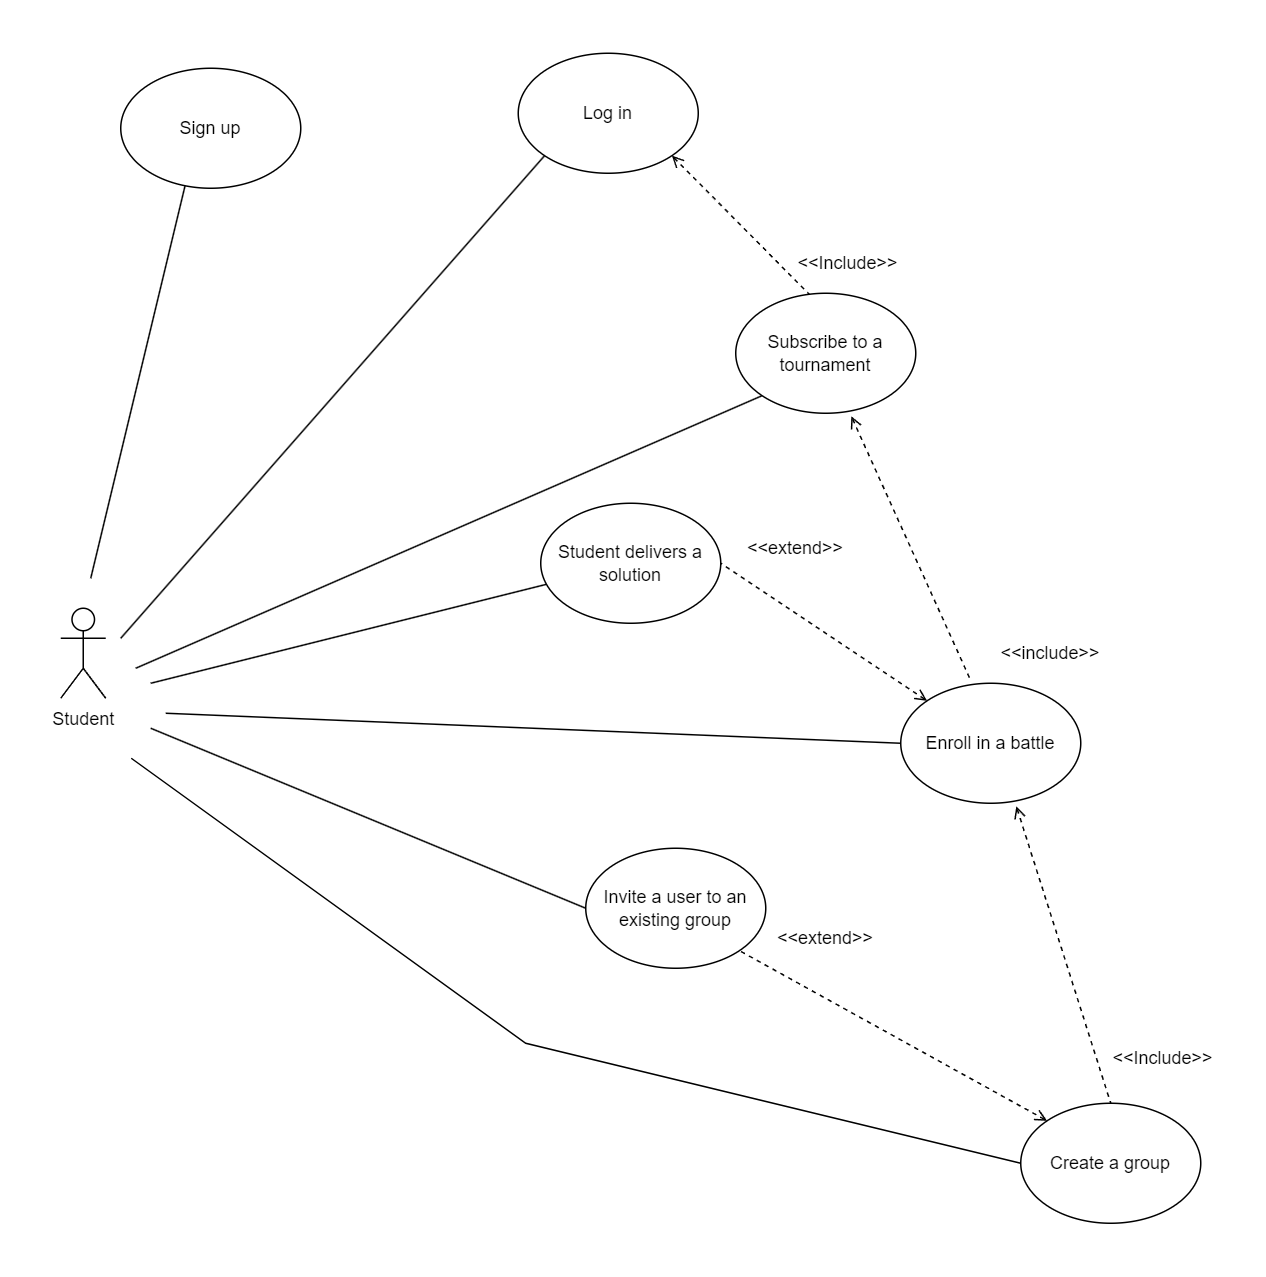
\includegraphics[width=1\textwidth]{../assets/section_3/StudentDiagram.png}
        \end{figure}
    \newpage
    \restoregeometry
    \begin{figure}[h!]
        \centering
        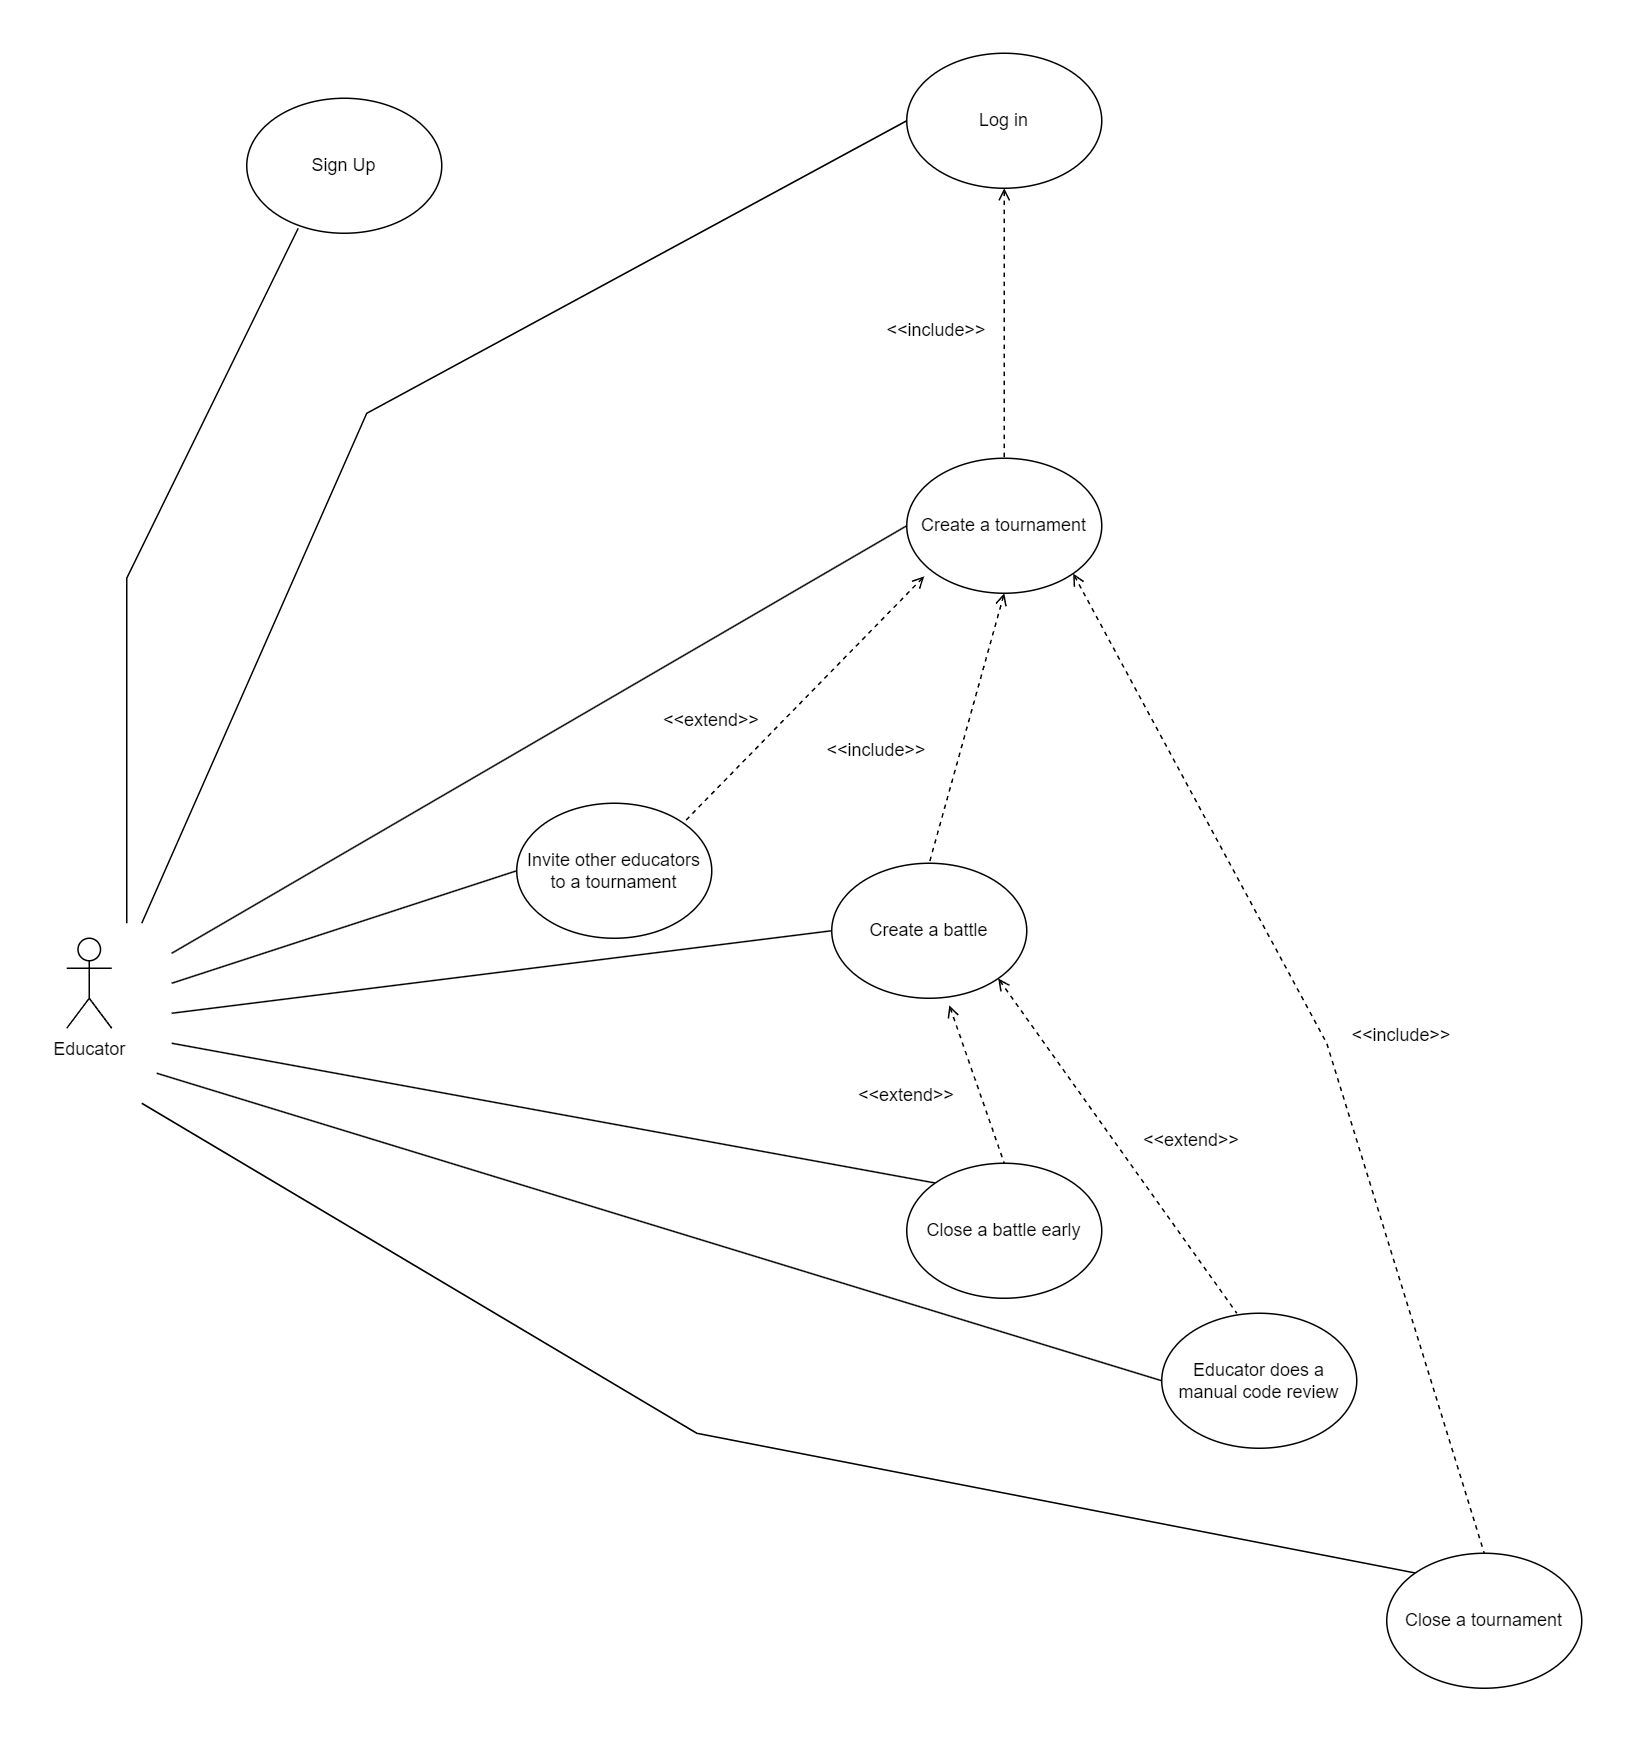
\includegraphics[width=1\textwidth]{../assets/section_3/EducatorDiagram.png}
    \end{figure}
    \newpage

    \subsubsection{Use cases}
    \textbf{Sign up}
        \begin{table}[H]
            \begin{center}
                \begin{tabular}{|m{10em}|m{30em}|}
                \hline
                \textbf{Use Case} & Sign up\\
                \hline
                \textbf{Actor} & User\\
                \hline
                \textbf{Entry condition} & User wants to register in the system\\
                \hline
                \textbf{Flow of events} & 
                    \begin{enumerate}
                        \item User accesses the application
                        \item User presses the sign-up button
                        \item User inserts his email and password
                        \item User presses the confirmation button
                        \item System checks that the e-mail has not been used before and that the password satisfy the security constraints
                        \item System displays a confirmation message
                        \item System sends a notification to User to confirm the successful registration
                    \end{enumerate}\\
                \hline
                \textbf{Exit condition} & User data are saved into the system and the registration ends successfully\\
                \hline
                \textbf{Exceptions} &
                Possible exceptions:
                \begin{enumerate}
                    \item User email has already been taken
                    \item User presses the cancel button after having pressed the sign-up button
                    \item The application is currently unavailable
                \end{enumerate}
                If one of these exceptions takes place, an error message is shown and the flow of events starts again from point 3\\
                \hline
                \end{tabular}
            \end{center}
        \end{table}\newpage

        \textbf{Log in}
        \begin{table}[ht]
            \begin{center}
                \begin{tabular}{|m{10em}|m{30em}|}
                \hline
                \textbf{Use Case} & Log in\\
                \hline
                \textbf{Actor} & User\\
                \hline
                \textbf{Entry condition} & User wants to log into the application\\
                \hline
                \textbf{Flow of events} & 
                    \begin{enumerate}
                        \item User accesses the application
                        \item User presses the login button
                        \item User enters his email and password
                        \item User presses the confirmation button
                        \item System displays the main page
                    \end{enumerate}\\
                \hline
                \textbf{Exit condition} & The system allows the user's to access the desired account and the main page is displayed\\
                \hline
                \textbf{Exceptions} & 
                Possible exceptions:
                \begin{enumerate}
                    \item The inserted email does not correspond to any account
                    \item The password for the given email is incorrect
                \end{enumerate}
                An error message is shown and the flow of events
                starts again from point 3\\
                \hline
                \end{tabular}
            \end{center}
        \end{table}\newpage

        \textbf{Create a tournament}
        \begin{table}[H]
            \begin{center}
                \begin{tabular}{|m{10em}|m{30em}|}
                \hline
                \textbf{Use Case} & Create a tournament\\
                \hline
                \textbf{Actor} & Educator\\
                \hline
                \textbf{Entry condition} & Educator wants to create a new tournament\\
                \hline
                \textbf{Flow of events} & 
                    \begin{enumerate}
                        \item Educator accesses the application
                        \item Educator logs-in
                        \item Educator navigates to the tournament section
                        \item Educator clicks the "Create a new Tournament" button
                        \item Educator inserts the name of the new tournament
                        \item Educator inserts the deadline of the new tournament
                        \item Educator press the "Create tournament" button
                        \item System checks if a tournament with the same name does already exist
                        \item System sends a confirmation notification of tournament creation to Educator
                        \item System sends a notification that a tournament with that name has been created to all CodeKata's users
                    \end{enumerate}\\
                \hline
                \textbf{Exit condition} & A new tournament with the required name has been successfully created and all users of the platform have notified about it\\
                \hline
                \textbf{Exceptions} & 
                    Possible exceptions:
                    \begin{enumerate}
                        \item A tournament with the same name does already exist
                    \end{enumerate}
                    The system shows an error message and the flow of events starts again from point 5\\
                \hline
                \end{tabular}
            \end{center}
        \end{table}\newpage

        \textbf{Invite other educators to manage a tournament}\\
        \begin{table}[h!]
            \begin{center}
                \begin{tabular}{|m{10em}|m{30em}|}
                \hline
                \textbf{Use Case} & Invite other educators to manage a tournament\\
                \hline
                \textbf{Actors} & 
                    \begin{itemize}
                        \item Tournament Owner
                        \item Educator(s)
                    \end{itemize}\\
                \hline
                \textbf{Entry condition} & Tournament Owner is logged in and wants to invite one or more educator(s) to manage one of his/her tournaments\\
                \hline
                \textbf{Flow of events} & 
                \begin{enumerate}
                    \item Tournament Owner clicks on "Tournament" page
                    \item Tournament Owner clicks on his/her tournament to which he/she wants to invite the educator(s) to
                    \item Tournament Owner clicks on "Manage educators" button
                    \item Tournament Owner clicks on the "+" button
                    \item Tournament Owner writes the name of the educator(s) that he/she wants to invite, after writing each of them he/she press the add button
                    \item Tournament Owner clicks the "Invite educators" button to confirm his choices
                    \item System notifies the educators previously selected about the fact that they have been invited to manage a tournament
                \end{enumerate}\\
                \hline
                \textbf{Exit condition} & The educator(s) have been correctly invited to manage the tournament and they have received a notification about it\\
                \hline
                \textbf{Exceptions} & 
                    Possible exceptions:
                    \begin{enumerate}
                        \item A written educator name does not exist
                    \end{enumerate}
                    The system shows an error message and the flow of events starts again from point 5\\
                \hline
                \end{tabular}
            \end{center}
        \end{table}\newpage

        \newgeometry{top=1em}
        \textbf{Create a battle}
        \begin{table}[H]
            \begin{center}
                \begin{tabular}{|m{10em}|m{30em}|}
                \hline
                \textbf{Use Case} & Create a battle\\
                \hline
                \textbf{Actor} & Educator\\
                \hline
                \textbf{Entry condition} & An educator managing a tournament is logged in and wants to create a battle in such tournament\\
                \hline
                \textbf{Flow of events} & 
                    \begin{enumerate}
                        \item Educator navigates to the "Tournament" section
                        \item Educator selects the tournament where he/she wants to create a new battle in
                        \item Educator clicks on the "New Battle" button
                        \item Educator clicks on "Upload" button in order to upload the code kata
                        \item Educator uploads the corresponding CodeKata
                        \item Educator fills up, using the provided fields, all the required information to create a new battle, which are:
                            \begin{itemize}
                                \item minimum number of students per group
                                \item maximum number of students per group
                                \item registration deadline
                                \item final submission deadline
                                \item which aspects of the quality level of the sources should be automatically evaluated
                                \item whether a manual evaluation will be needed after the automated one
                            \end{itemize}
                        \item Educator clicks on "Create new battle" button
                        \item System notifies all students subscribed to the tournament that a battle has been created
                    \end{enumerate}\\
                \hline
                \textbf{Exit condition} & A new battle has been created with the desired configuration and all students subscribed to its tournament have been notified about it\\
                \hline
                \textbf{Exceptions} & 
                    Possible exceptions:
                    \begin{enumerate}
                        \item Some configuration fields are left empty
                        \item Some configuration fields are filled with incorrect values (for example a negative value for the maximum number of students per group)
                    \end{enumerate}
                    The system shows an error message and the flow of events starts again from point 6\\
                \hline
                \end{tabular}
            \end{center}
        \end{table}\newpage

        \restoregeometry
        \textbf{Subscribe to a tournament}
        \begin{table}[ht]
            \begin{center}
                \begin{tabular}{|m{10em}|m{30em}|}
                \hline
                \textbf{Use Case} & Subscribe to a tournament\\
                \hline
                \textbf{Actor} & User\\
                \hline
                \textbf{Entry condition} & A logged-in user wants to subscribe to a tournament\\
                \hline
                \textbf{Flow of events} & 
                    \begin{enumerate}
                        \item User navigates to the tournament section
                        \item User clicks on the tournament name of the tournament to which he/she wants to subscribe to
                        \item User clicks on the "Subscribe" button
                    \end{enumerate}\\
                \hline
                \textbf{Exit condition} & The user is subscribed to the tournament he/she wanted to, and now he/she will be informed about every new battle created in that tournament\\
                \hline
                \end{tabular}
            \end{center}
        \end{table}\newpage

        \newgeometry{top=8em}
        \textbf{Create Group}
        \begin{table}[h!]
            \begin{center}
                \begin{tabular}{|m{10em}|m{30em}|}
                \hline
                \textbf{Use Case} & Create Group\\
                \hline
                \textbf{Actor} & Student\\
                \hline
                \textbf{Entry condition} & A logged in student wants to create a group in the context of a battle to which he/she is enrolled\\
                \hline
                \textbf{Flow of events} & 
                    \begin{enumerate}
                        \item Student navigates to the tournament section
                        \item Student clicks on the tournament name in which he/she wants to create a group
                        \item Student clicks on the "Create a group" button
                        \item System checks if there is an ongoing battle and if the user is enrolled into such battle
                        \item Student inserts in the corresponding field the name of the new group
                        \item Student clicks on the "Confirm Creation" button
                        \item System check if the name of the group is already used in the context of the same battle
                        \item System shows a confirmation message about the successful group creation
                    \end{enumerate}\\
                \hline
                \textbf{Exit condition} & The new group has been created with the corresponding name\\
                \hline
                \textbf{Exceptions} & 
                    Possible exceptions:
                    \begin{enumerate}
                        \item In this tournament there is no current ongoing battle
                        \item There already exist a group with the same name in the context of that battle
                    \end{enumerate}
                    The system shows an error message and the flow of events starts again from point 2 if exception 1 has occurred and from point 5 if exception 2 has occurred\\
                \hline
                \end{tabular}
            \end{center}
        \end{table}\newpage
        \restoregeometry

        \textbf{Invite a student to an existing group}
        \begin{table}[h!]
            \begin{center}
                \begin{tabular}{|m{10em}|m{30em}|}
                \hline
                \textbf{Use Case} & Invite a student to an existing group\\
                \hline
                \textbf{Actors} & 
                    \begin{itemize}
                        \item Group Student
                        \item New Student
                    \end{itemize}\\
                \hline
                \textbf{Entry condition} & A logged in student which has already created a group for a tournament he/she is subscribed to (Group Student), wants to invite another student which is also subscribed to such tournament to his/her group (New Student)\\
                \hline
                \textbf{Flow of events} & 
                    \begin{enumerate}
                        \item Group Student navigates to the tournament section
                        \item Group Student clicks on the tournament name in which such group has been created
                        \item Group Student clicks on the "Manage my group" button
                        \item Group Student clicks on the "Invite new student" button
                        \item Group Student write the nickname or the email of New Student
                        \item Group Student clicks the "Invite" button
                        \item System sends a notification to New Student about his invitation to such group
                    \end{enumerate}\\
                \hline
                \textbf{Exit condition} & 
                    New Student is successfully invited to the existing group and has been notified about it\\
                \hline
                \textbf{Exceptions} & 
                    Possible exceptions:
                    \begin{enumerate}
                        \item The nickname/email written doesn't correspond to any user
                        \item The invited user is not subscribed to such tournament
                    \end{enumerate}
                    The system shows an error message and the flow of events starts again from point 4\\
                \hline
                \end{tabular}
            \end{center}
        \end{table}\newpage

        \textbf{Enroll in a battle}
        \begin{table}[ht]
            \begin{center}
                \begin{tabular}{|m{10em}|m{30em}|}
                \hline
                \textbf{Use Case} & Enroll in a battle\\
                \hline
                \textbf{Actor} & Student\\
                \hline
                \textbf{Entry condition} & A logged in student wants to enroll in a battle\\
                \hline
                \textbf{Flow of events} &
                    \begin{enumerate}
                        \item Student navigates to the tournament section
                        \item Student clicks on the tournament name of the tournament in which there is the battle to which he/she wants to enroll into
                        \item Student clicks on the current ongoing battle
                        \item Student clicks on the "Enroll into battle" button
                        \item System checks that the group of the student satisfy all the constraints required by the specific battle
                        \item System shows a confirmation message about the successful enrollment into that battle
                    \end{enumerate}\\
                \hline
                \textbf{Exit condition} & Student and possibly his/her group are enrolled into the battle\\
                \hline
                \textbf{Exceptions} & 
                    Possible exceptions:
                    \begin{enumerate}
                        \item The student's group doesn't satisfy that battle's constraints
                    \end{enumerate}
                    The system shows an error message and the flow of events starts again from point 3\\
                \hline
                \end{tabular}
            \end{center}
        \end{table}\newpage

        \textbf{Student delivers a solution}
        \begin{table}[ht]
            \begin{center}
                \begin{tabular}{|m{10em}|m{30em}|}
                \hline
                \textbf{Use Case} & Student delivers a solution\\
                \hline
                \textbf{Actor} & Student\\
                \hline
                \textbf{Entry condition} & A logged in student wants to deliver their shared solution  or his/her personal solution of a certain active battle\\
                \hline
                \textbf{Flow of events} & 
                    \begin{enumerate}
                        \item Student set up an automated procedure, using the repository system that informs the CKB platform when a push action occurs
                        \item Student commits the change that he/she has made to the source code
                        \item Student push their shared solution to the repository
                    \end{enumerate}\\
                \hline
                \textbf{Exit condition} & The solution made by such group has been delivered and CKB has been informed about this delivery\\
                \hline
                \end{tabular}
            \end{center}
        \end{table}\newpage

        \textbf{Educator does a manual code review}
        \begin{table}[h!]
            \begin{center}
                \begin{tabular}{|m{10em}|m{30em}|}
                \hline
                \textbf{Use Case} & Educator does a manual code review\\
                \hline
                \textbf{Actor} & Educator\\
                \hline
                \textbf{Entry condition} & A battle has ended and the educator when creating this battle set up that a manual evaluation was needed after the automated ones\\
                \hline
                \textbf{Flow of events} & 
                    \begin{enumerate}
                        \item Educator navigates to the tournament section
                        \item Educator selects the tournament in which the battle awaiting a manual delivery has been created
                        \item Educator selects the battle requiring a manual evaluation
                        \item Educator clicks on the "Review submissions" button
                        \item The system presents to the educator the first delivery that has been submitted, by alphabetical order of the name of the group that submitted it along with the result of its automated evaluations
                        \item Educator read the whole code and gives his/her personal evaluation to the delivery
                        \item Educator presses the "Next One" button
                    \end{enumerate}\\
                \hline
                \textbf{Exit condition} & 
                    The delivery has received a manual evaluation\\
                \hline
                \textbf{Exceptions} & 
                    Possible exceptions:
                    \begin{enumerate}
                        \item Educator presses the "Next one" button before having given his/her personal evaluation
                    \end{enumerate}
                    The system shows an error message and the flow of events starts again from point 4\\
                \hline
                \end{tabular}
            \end{center}
        \end{table}\newpage

        \textbf{Close a battle early}
        \begin{table}[ht]
            \begin{center}
                \begin{tabular}{|m{10em}|m{30em}|}
                \hline
                \textbf{Use Case} & Close a battle early\\
                \hline
                \textbf{Actor} & Educator\\
                \hline
                \textbf{Entry condition} & A logged in educator wants to close one of his/her battles before its expected conclusion\\
                \hline
                \textbf{Flow of events} & 
                    \begin{enumerate}
                        \item Educator navigates to the tournament section \item Educator selects the tournament in which he has previously created such battle
                        \item Educator navigates to the current battle
                        \item Educator clicks on the "Delete battle" button
                        \item Educator clicks on the "Yes, I'm sure" button
                        \item System closes the corresponding battle
                    \end{enumerate}\\
                \hline
                \textbf{Exit condition} & 
                    The battle has been successfully removed early\\
                \hline
                \end{tabular}
            \end{center}
        \end{table}\newpage

        \textbf{Close a tournament}
        \begin{table}[ht]
            \begin{center}
                \begin{tabular}{|m{10em}|m{30em}|}
                \hline
                \textbf{Use Case} & Close a tournament\\
                \hline
                \textbf{Actor} & Educator\\
                \hline
                \textbf{Entry condition} & A logged in educator wants to close one of his/her tournament\\
                \hline
                \textbf{Flow of events} & 
                    \begin{enumerate}
                        \item Educator navigates to the tournament section \item Educator selects the tournament he/she wants to close
                        \item Educator clicks on the "Close tournament" button
                        \item Educator clicks on the "Yes, I'm sure" button
                        \item System closes the corresponding tournament
                    \end{enumerate}\\
                \hline
                \textbf{Exit condition} & The educator's tournament has been closed\\
                \hline
                \textbf{Exceptions} & 
                    Possible exceptions:
                    \begin{enumerate}
                        \item The tournament has an ongoing battle
                    \end{enumerate}
                    The system shows an error message and the flow of events starts again from point 2\\
                \hline
                \end{tabular}
            \end{center}
        \end{table}\newpage

    \newgeometry{top=6em}
    \subsubsection*{Traceability Matrix}
    \begin{table}[h!]
        \begin{center}
            \begin{tabular}{|m{10em}|m{30em}|}
            \hline
            \rowcolor{UCMappingFirstRow}
            \textbf{Use case} & \textbf{Requirement ID}\\
            \hline
            Sign up \cellcolor{UCMappingFirstColumn}& \textbf{R1:} The system must allow the registration of new users using their e-mail\cellcolor{UCMappingSecondColumn}\newline
            \textbf{R2:} The system must notify a user about his/her successful registration\cellcolor{UCMappingSecondColumn}\newline
            \textbf{R5:} The system must respect the GDPR\cellcolor{UCMappingSecondColumn}\\
            \hline
            Log in \cellcolor{UCMappingFirstColumn}& \textbf{R3:} The system must allow registered users to log-in using their e-mail\cellcolor{UCMappingSecondColumn}\newline
            \textbf{R4:} The system must allow logged-in users to use the application\cellcolor{UCMappingSecondColumn}\\
            \hline
            Create a tournament \cellcolor{UCMappingFirstColumn}& \textbf{R8:} The system must allow an educator to create a tournament if another tournament with the same name doesn't already exist\cellcolor{UCMappingSecondColumn}\newline
            \textbf{R9:} The system must reject an educator request to create a tournament if another
            tournament with the same name already exist\cellcolor{UCMappingSecondColumn}\newline
            \textbf{R13:} The system must allow an educator to set a registration deadline when creating
            a tournament\cellcolor{UCMappingSecondColumn}\\
            \hline
            Invite other educators to manage a\newline tournament \cellcolor{UCMappingFirstColumn}& \textbf{R10:} The system must allow the owner of a tournament to invite other educators to manage it\cellcolor{UCMappingSecondColumn}\newline
            \textbf{R11:} The system must notify an educator when he/she is invited to manage a tournament\cellcolor{UCMappingSecondColumn}\newline
            \textbf{R12:} The system must allow an educator to accept the invitation of another educator to manage a tournament\cellcolor{UCMappingSecondColumn}\\
            \hline
            Create a battle \cellcolor{UCMappingFirstColumn}& \textbf{R14:} The system must allow to set a minimum number of students for each group when creating a new battle\cellcolor{UCMappingSecondColumn}\newline
            \textbf{R15:} The system must allow to set the maximum number of students for each group when creating a new battle\cellcolor{UCMappingSecondColumn}\newline
            \textbf{R16:} The system must allow to set a registration deadline when creating a new battle\cellcolor{UCMappingSecondColumn}\newline
            \textbf{R17:} The system must allow to set a final submission deadline when creating a new
            battle\cellcolor{UCMappingSecondColumn}\newline
            \textbf{R18:} The system must allow an educator to choose while creating a new battle which
            aspects of the quality level of the sources will be automatically evaluated\cellcolor{UCMappingSecondColumn}\newline
            \textbf{R19:} The system must allow an educator to choose while creating a new battle whether a manual evaluation will be needed after the automated ones\cellcolor{UCMappingSecondColumn}\newline
            \textbf{R20:} The system must be able to receive a new code kata from an educator when he/she is creating a battle\cellcolor{UCMappingSecondColumn}\newline
            \textbf{R23:} The system must notify all students subscribed to that tournament when a new battle of such tournament starts\cellcolor{UCMappingSecondColumn}\\
            \hline
            \end{tabular}
        \end{center}
    \end{table}
    \newpage
    \restoregeometry

    \begin{table}[h!]
        \begin{center}
            \begin{tabular}{|m{10em}|m{30em}|}
            \hline
            \rowcolor{UCMappingFirstRow}
            \textbf{Use case} & \textbf{Requirement ID}\\
            \hline
            Subscribe to a\newline tournament \cellcolor{UCMappingFirstColumn}& \textbf{R24:} The system must allow users to subscribe to a tournament\cellcolor{UCMappingSecondColumn}\\
            \hline
            Create group \cellcolor{UCMappingFirstColumn}& \textbf{R25:} The system must allow students to create groups in the context of a battle\cellcolor{UCMappingSecondColumn}\\
            \hline
            Enroll in a battle \cellcolor{UCMappingFirstColumn}& \textbf{R30:} The system must allow groups to join a newly created battle if they respect that
            battle's constraints\cellcolor{UCMappingSecondColumn}\\
            \hline
            Invite a student to an\newline existing group \cellcolor{UCMappingFirstColumn}& \textbf{R26:} The system must allow a student to invite another to his/her own group, if such student is enrolled into the corresponding battle\cellcolor{UCMappingSecondColumn}\newline
            \textbf{R27:} The system must reject a user request to invite another student to his/her own group, if such student is not enrolled into the corresponding battle\cellcolor{UCMappingSecondColumn}\newline
            \textbf{R28:} The system must notify a student when he/she is invited to a group\cellcolor{UCMappingSecondColumn}\newline
            \textbf{R29:} The system must allow a student to join an existing group if invited\cellcolor{UCMappingSecondColumn}\\
            \hline
            Student delivers a\newline solution \cellcolor{UCMappingFirstColumn} & \textbf{R32:} The system must allow a group to submit his/their solution\cellcolor{UCMappingSecondColumn}\\
            \hline
            Educator does a\newline manual code review \cellcolor{UCMappingFirstColumn}& \textbf{R40:} The system must show the results of its automated analysis to the educators managing the tournament\cellcolor{UCMappingSecondColumn}\newline
            \textbf{R41:} The system must allow an educator to see the solution provided by each group\cellcolor{UCMappingSecondColumn}\newline
            \textbf{R42:} The system must allow an educator to manually mark a solution in the consolidation phase, if this was set up in the initial configuration of the battle\cellcolor{UCMappingSecondColumn}\\
            \hline
            \end{tabular}
        \end{center}
    \end{table}
    \newpage

    \begin{table}[h!]
        \begin{center}
            \begin{tabular}{|m{10em}|m{30em}|}
            \hline
            \rowcolor{UCMappingFirstRow}
            \textbf{Use case} & \textbf{Requirement ID}\\
            \hline
            Close a battle early \cellcolor{UCMappingFirstColumn} & \textbf{R48:} The system must allow an educator to close a battle before its expected conclusion\cellcolor{UCMappingSecondColumn}\newline
            \textbf{R49:} The system must allow an educator to set up a message explaining his/her motivations when closing a battle ahead of time\cellcolor{UCMappingSecondColumn}\newline
            \textbf{R50:} The system must notify all users subscribed to its tournament when a battle is closed ahead of time\cellcolor{UCMappingSecondColumn}\newline
            \textbf{R51:} The system must show the educator's motivation message when notifying students about the early closure of a battle\cellcolor{UCMappingSecondColumn}\\
            \hline
            Close a tournament \cellcolor{UCMappingFirstColumn}& \textbf{R52:} The system must allow an educator to close a tournament, if there is not an ongoing battle in such tournament\cellcolor{UCMappingSecondColumn}\newline
            \textbf{R53:} The system must reject an educator request to close a tournament, if there is an ongoing battle in such tournament\cellcolor{UCMappingSecondColumn}\newline
            \textbf{R54:} The system must notify all students subscribed to a tournament when such tournament is closed\cellcolor{UCMappingSecondColumn}\\
            \hline
        \end{tabular}
    \end{center}
    \end{table}
    \newpage

    \subsubsection{Sequence Diagrams}
    \textbf{Sign up}
    \begin{figure}[h!]
        \centering
        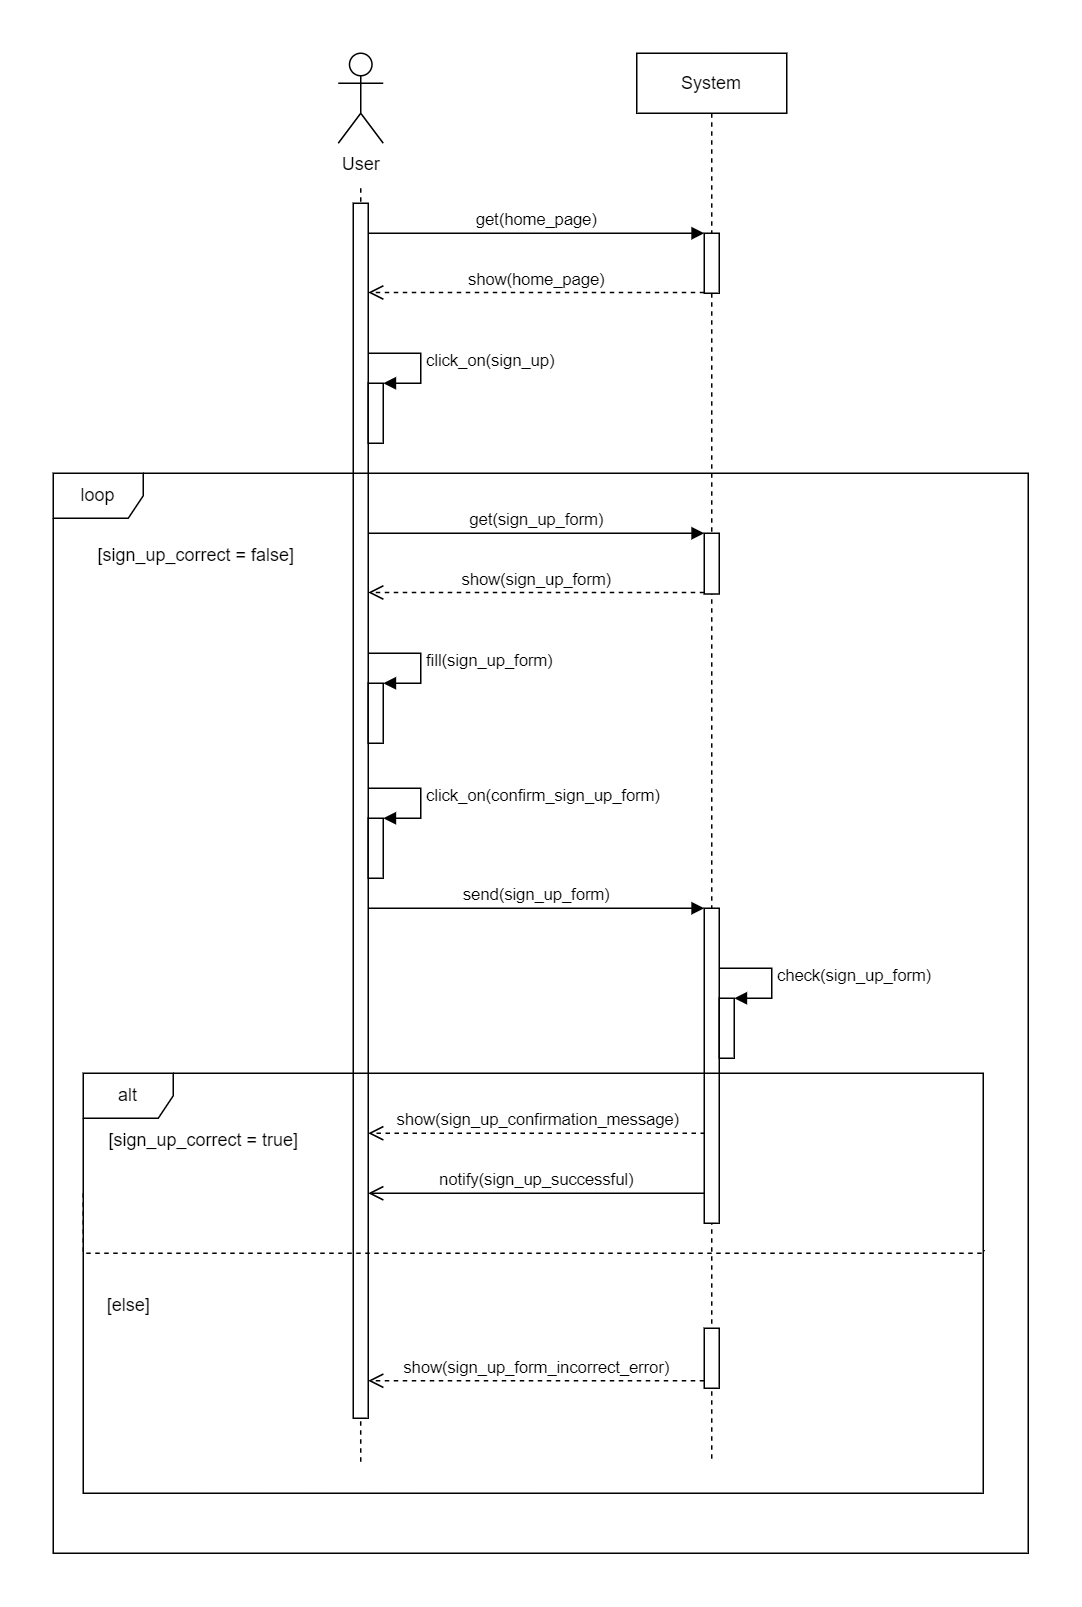
\includegraphics[width=0.75\textwidth]{../assets/section_3/SignUpDiagram.png}
    \end{figure}\\
    \newpage

    \textbf{Log in}
    \begin{figure}[h!]
        \centering
        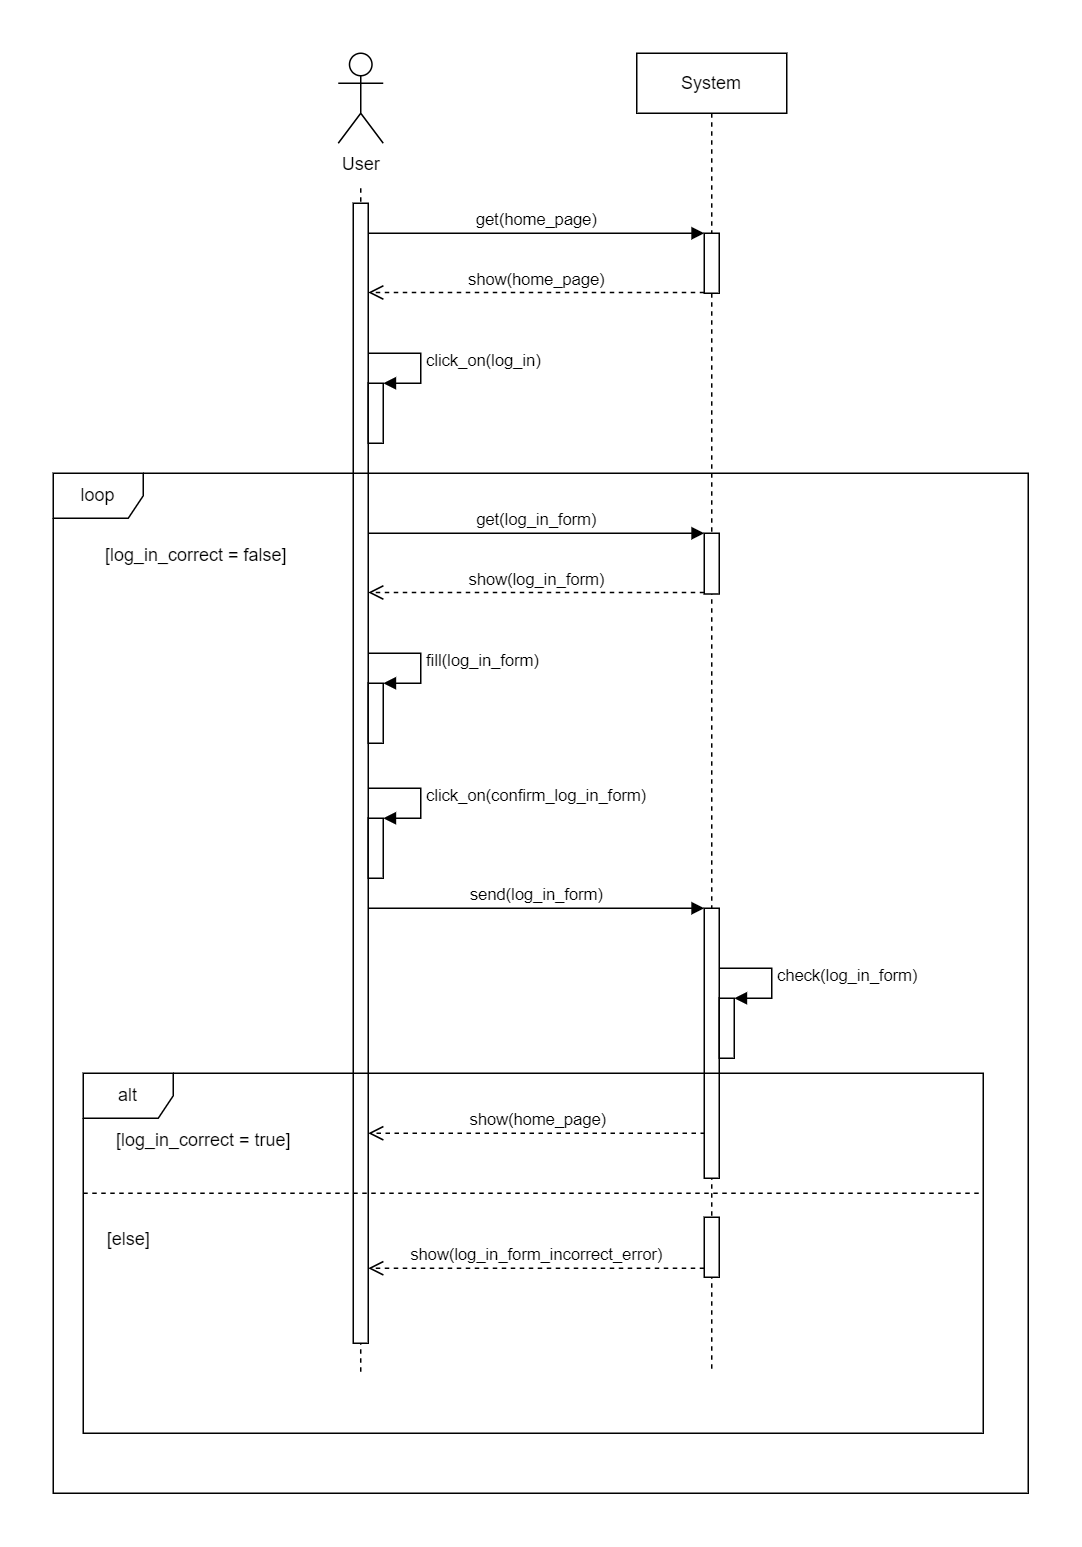
\includegraphics[width=0.85\textwidth]{../assets/section_3/LoginDiagram.png}
    \end{figure}
    \newpage

    \textbf{Create a tournament}
    \begin{figure}[h!]
        \centering
        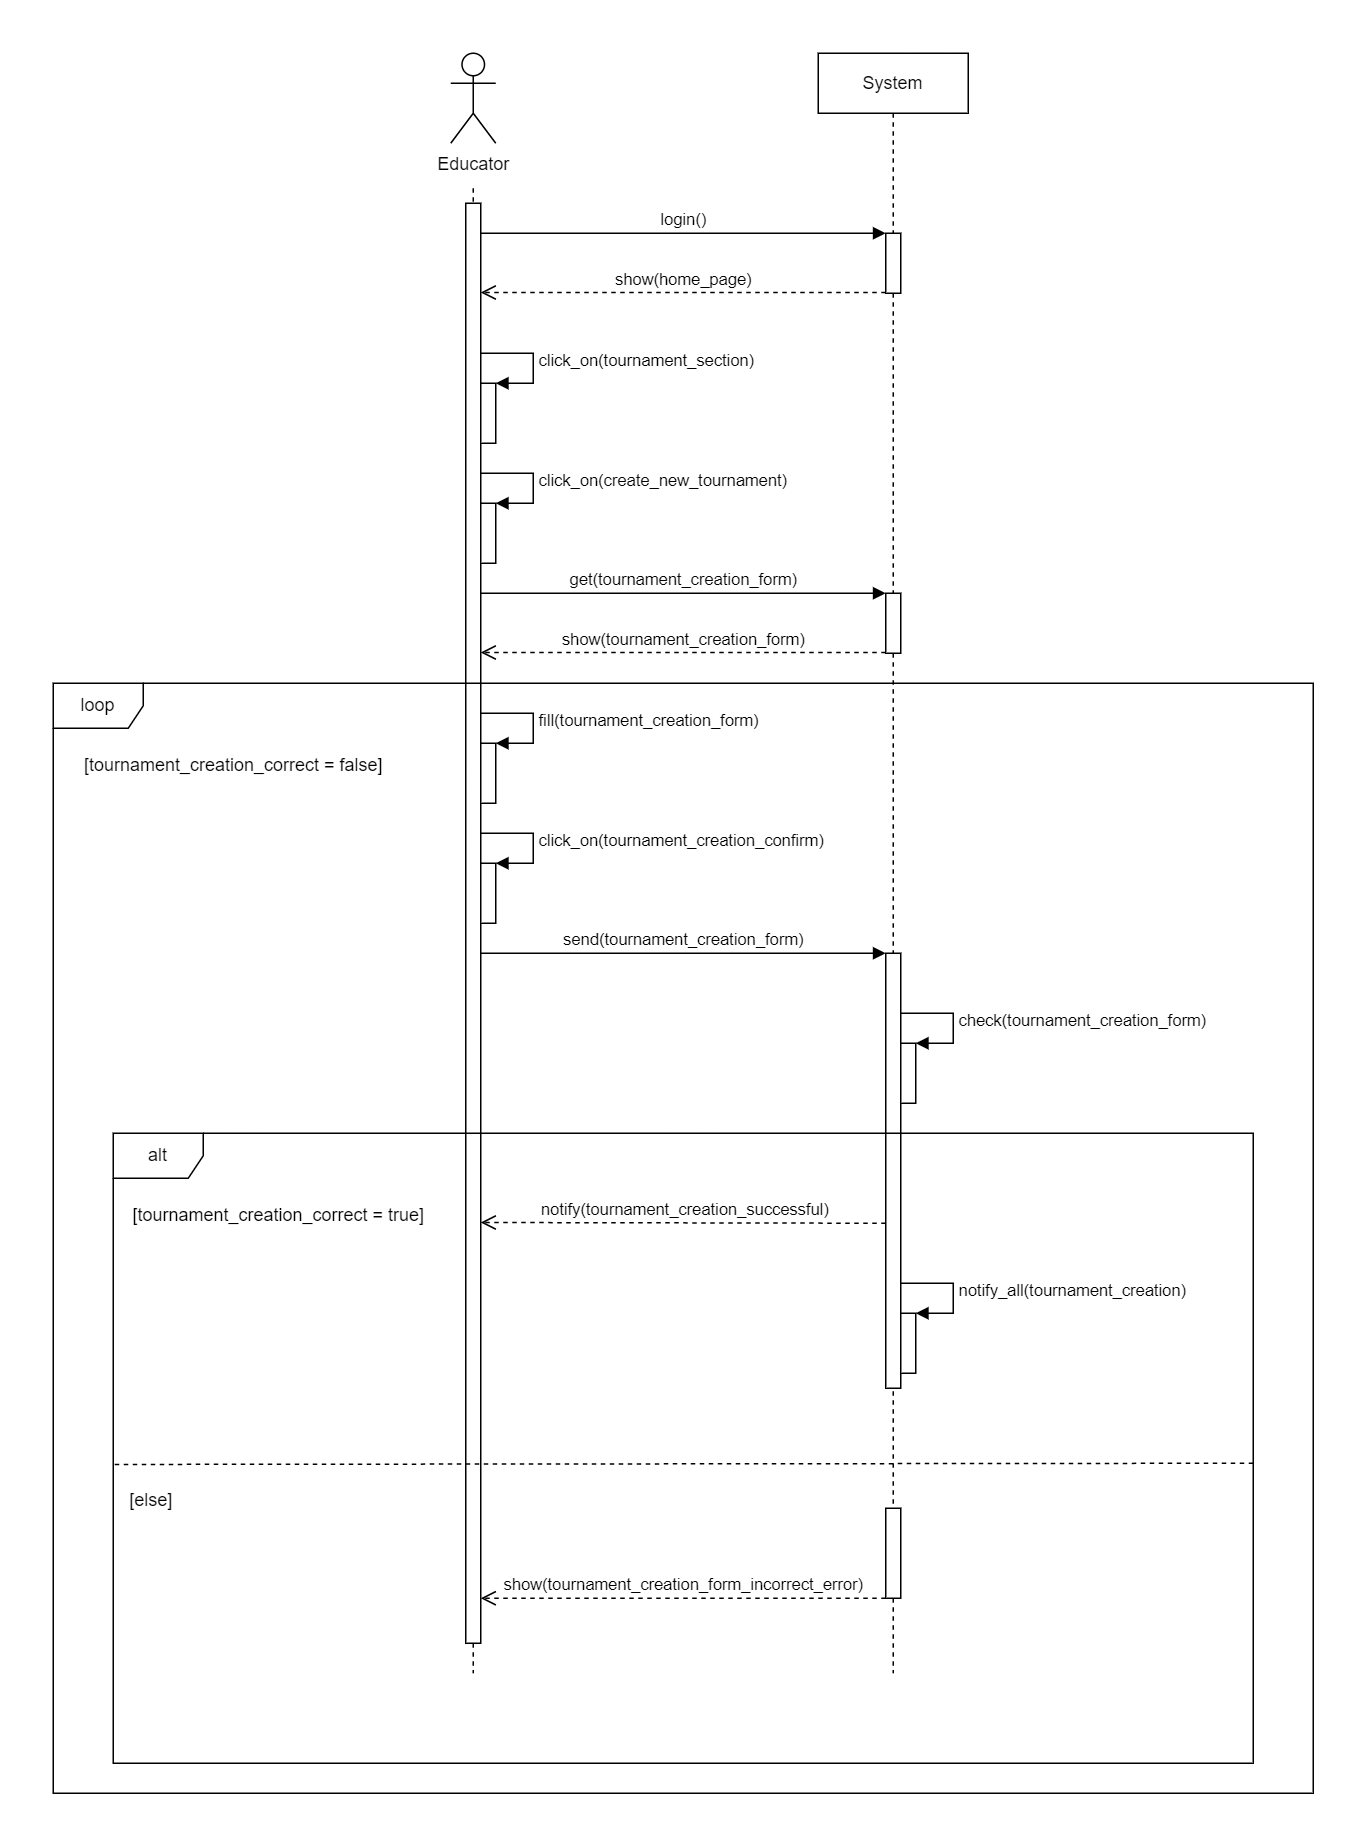
\includegraphics[width=0.9\textwidth]{../assets/section_3/CreateATournamentDiagram.png}
    \end{figure}
    \newpage

    \newgeometry{top=2em}
    \textbf{Invite other educators to mange a tournament}
    \begin{figure}[h!]
        \centering
        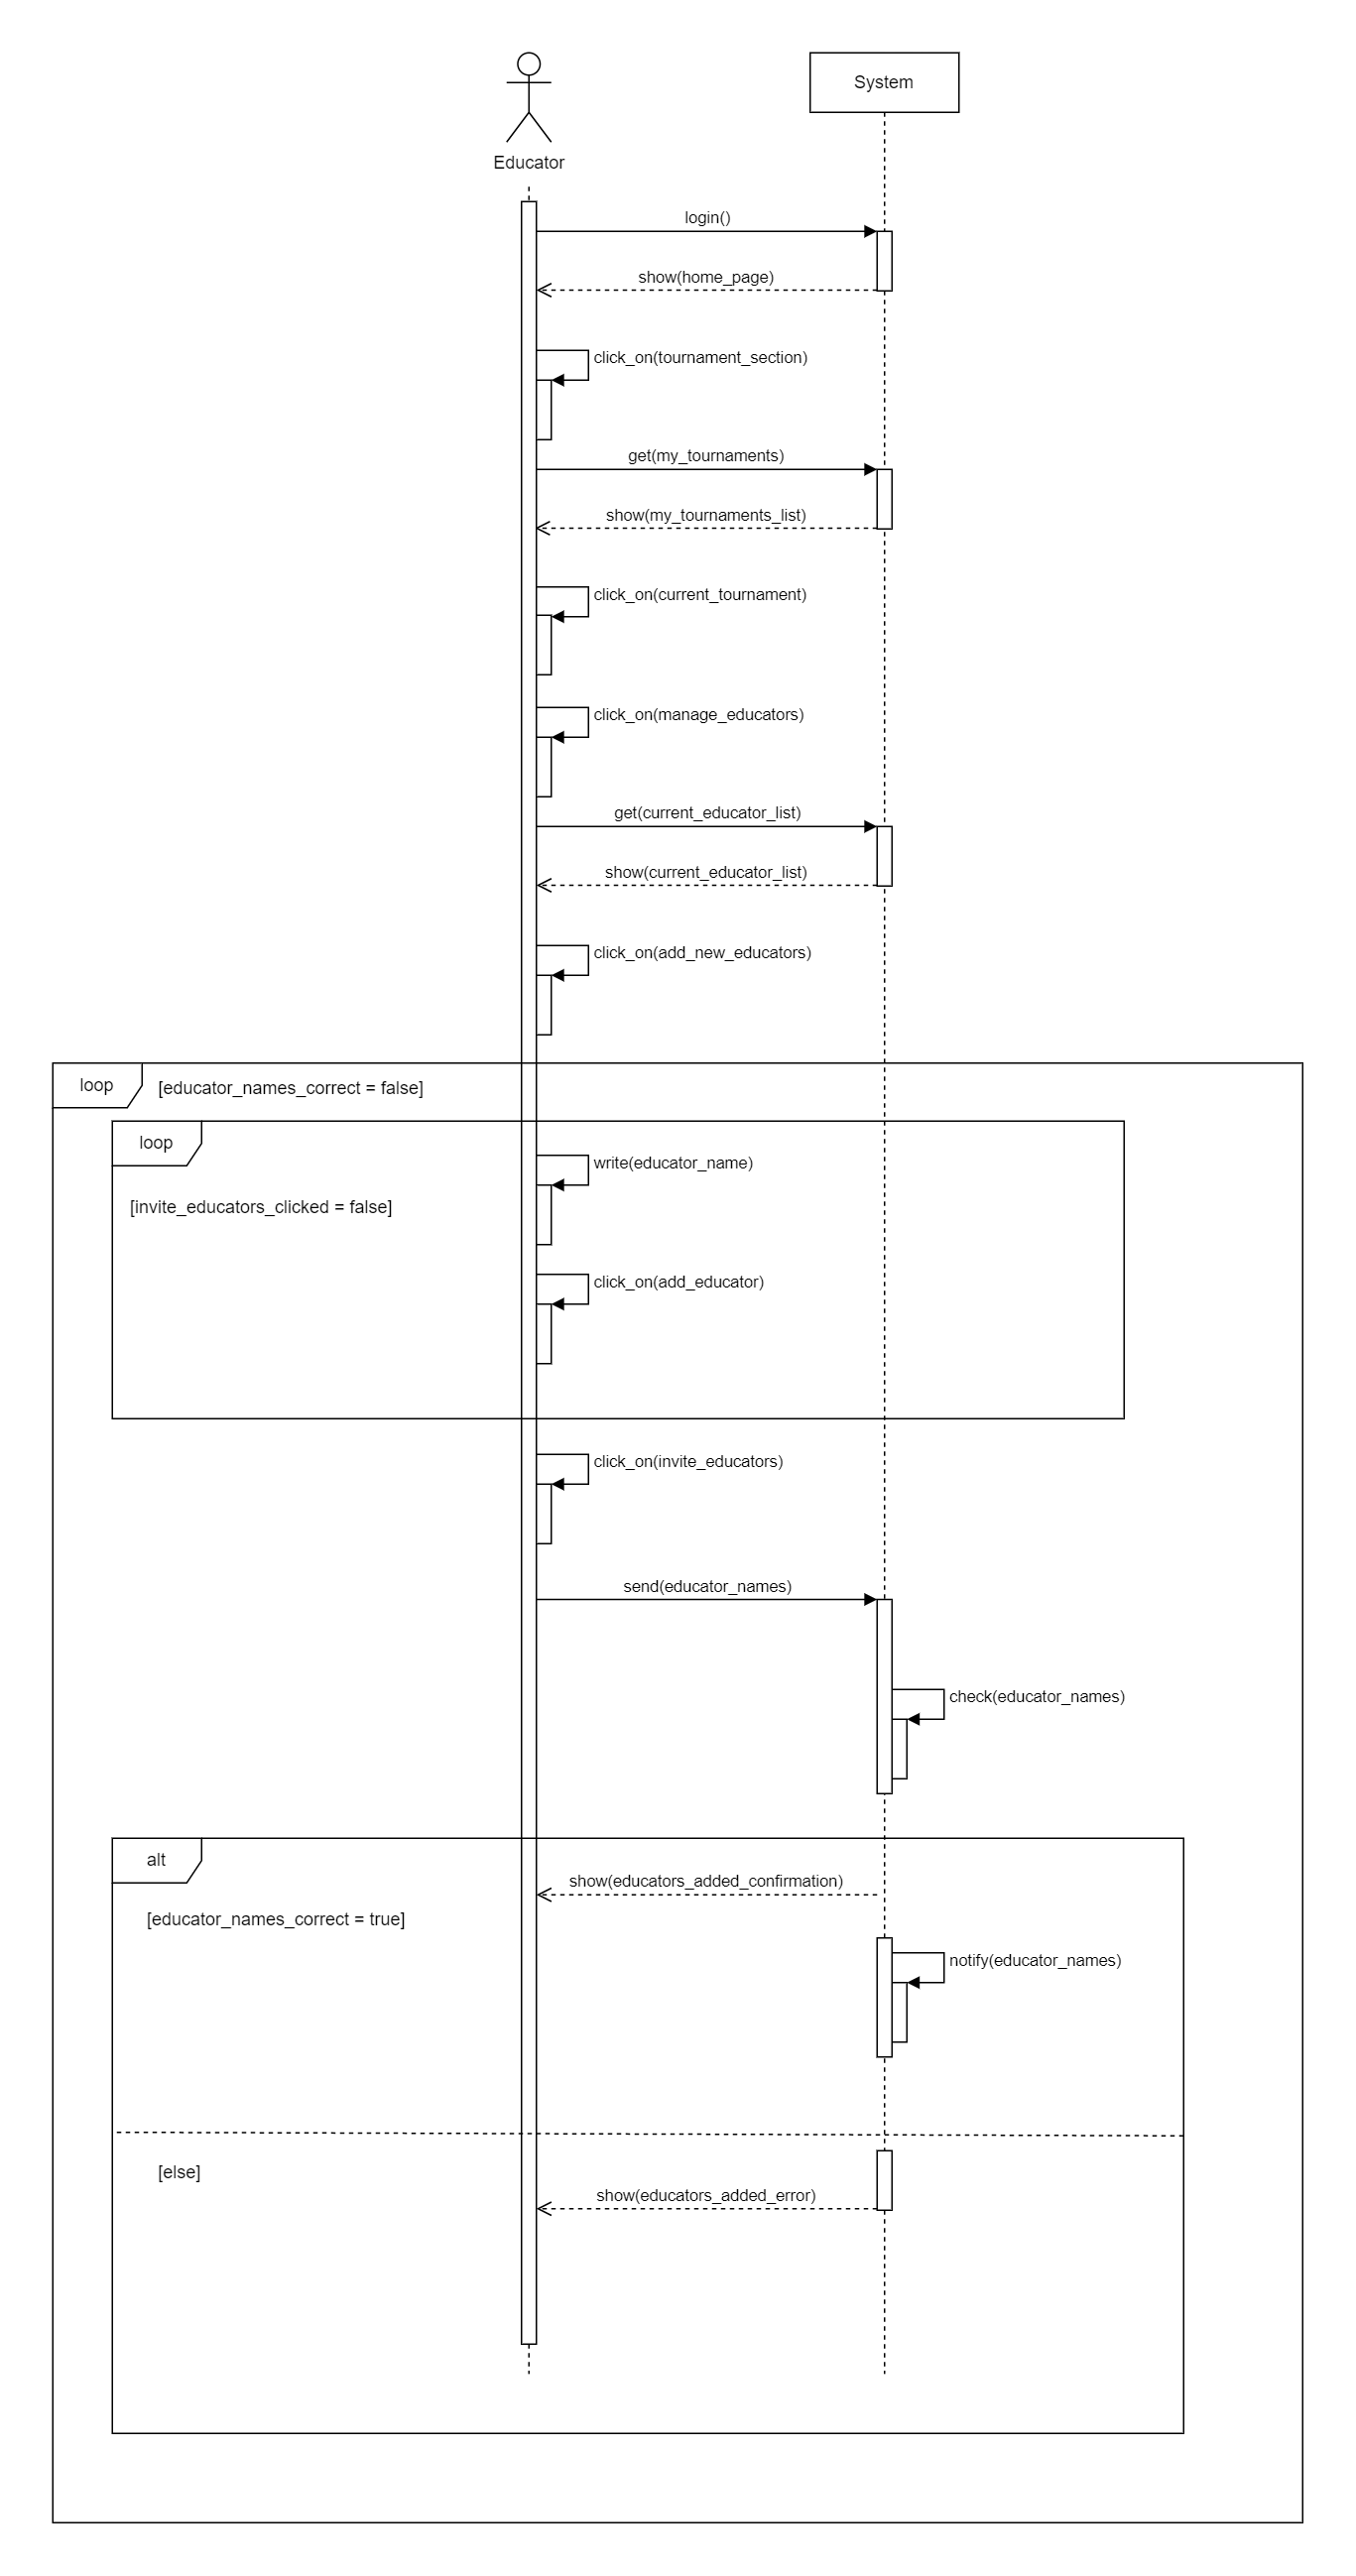
\includegraphics[width=0.79\textwidth]{../assets/section_3/InviteOtherEducatorsToManageATournament.png}
    \end{figure}
    \newpage
    \restoregeometry

    \newgeometry{top=3em}
    \textbf{Create a battle}
    \begin{figure}[h!]
        \centering
        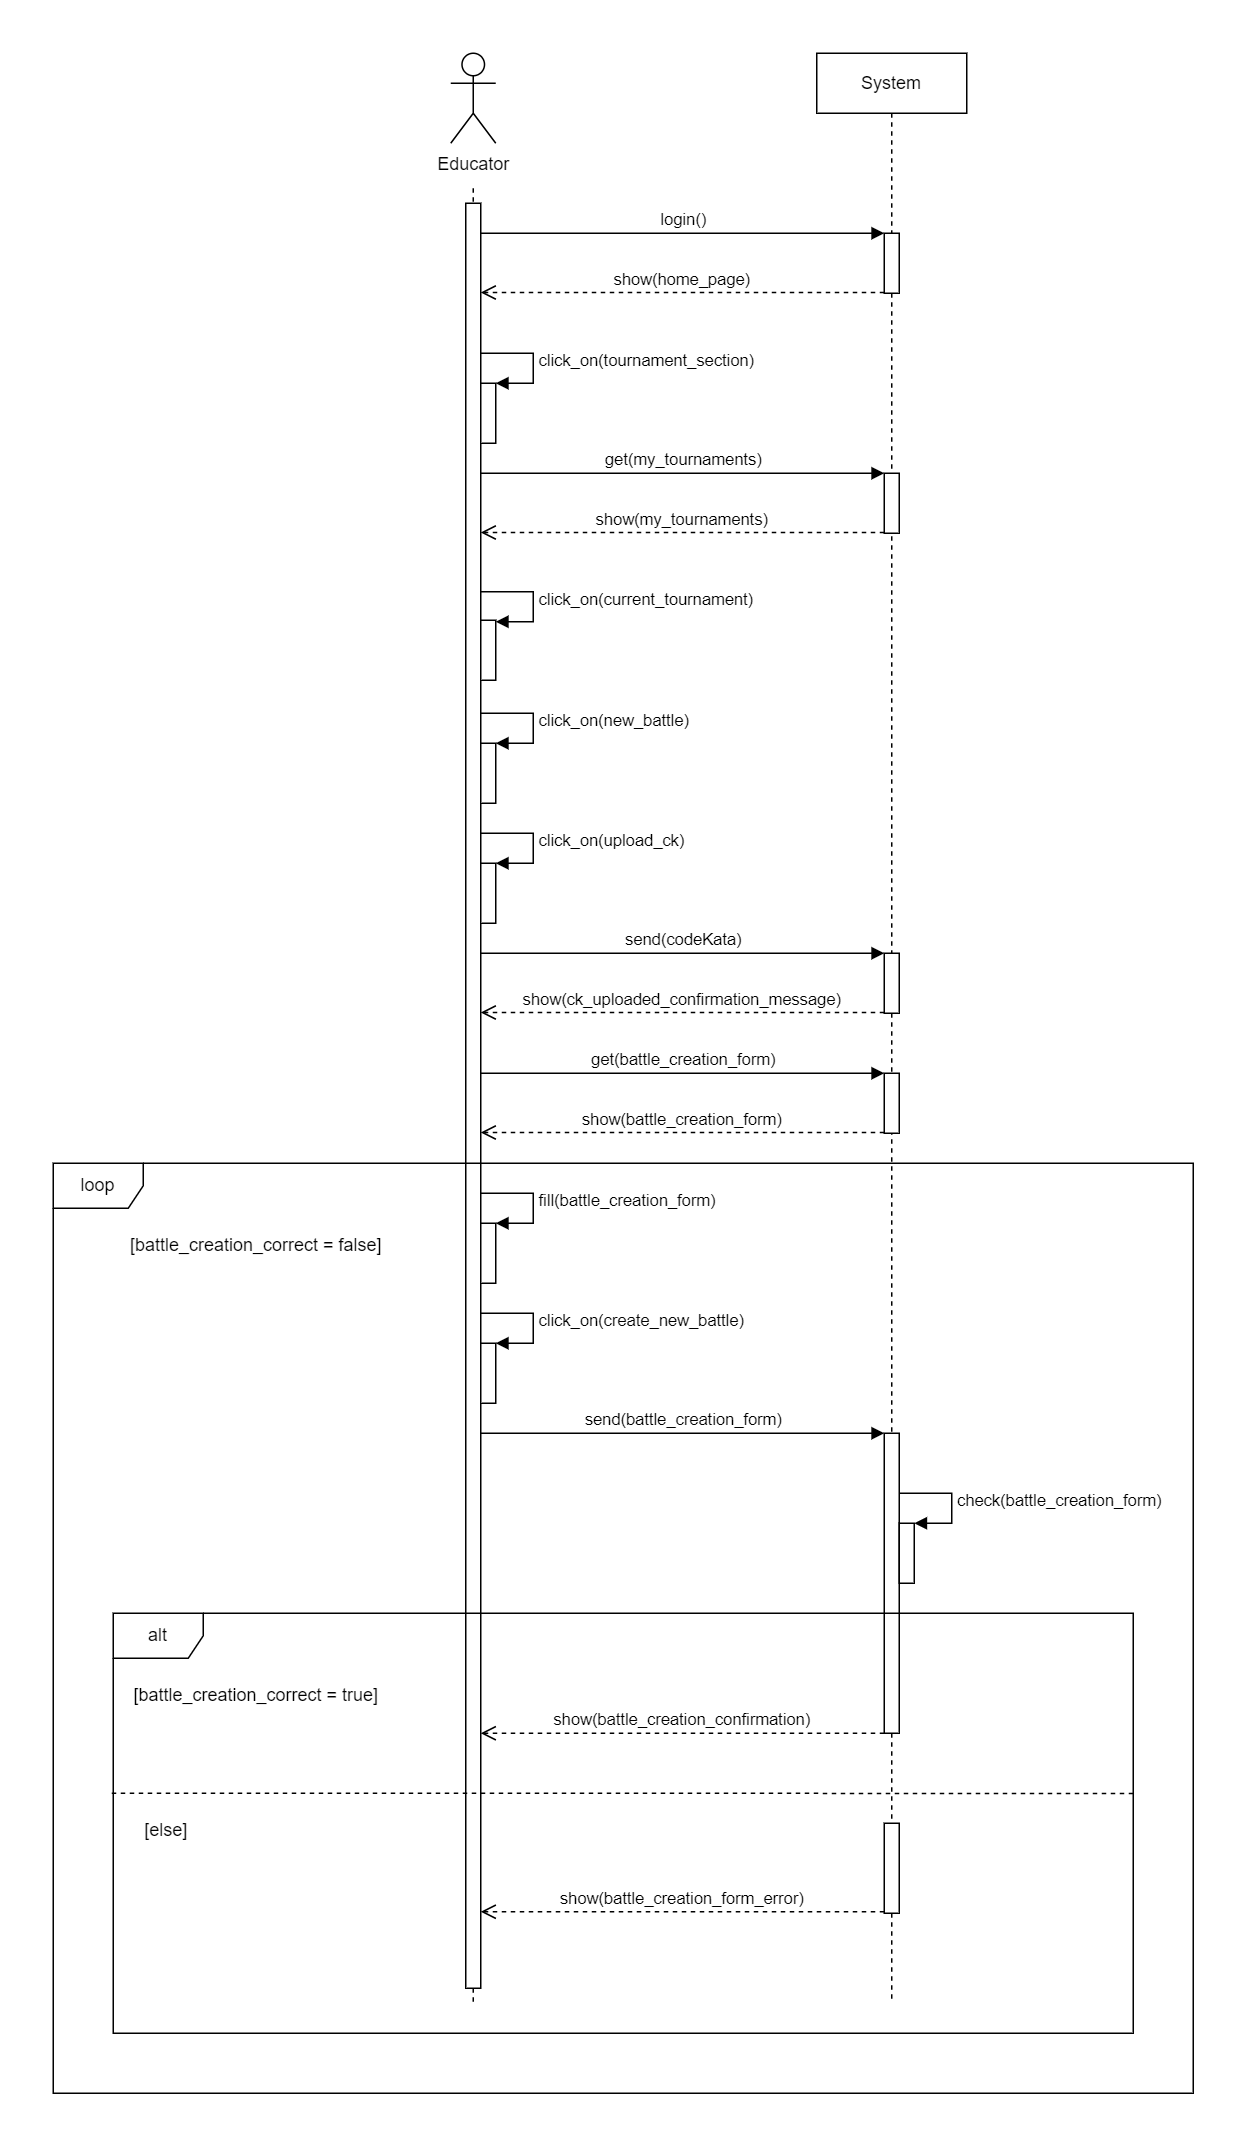
\includegraphics[width=0.85\textwidth]{../assets/section_3/CreateABattle.png}
    \end{figure}
    \newpage
    \restoregeometry

    \textbf{Subscribe to a tournament}
    \begin{figure}[H]
        \centering
        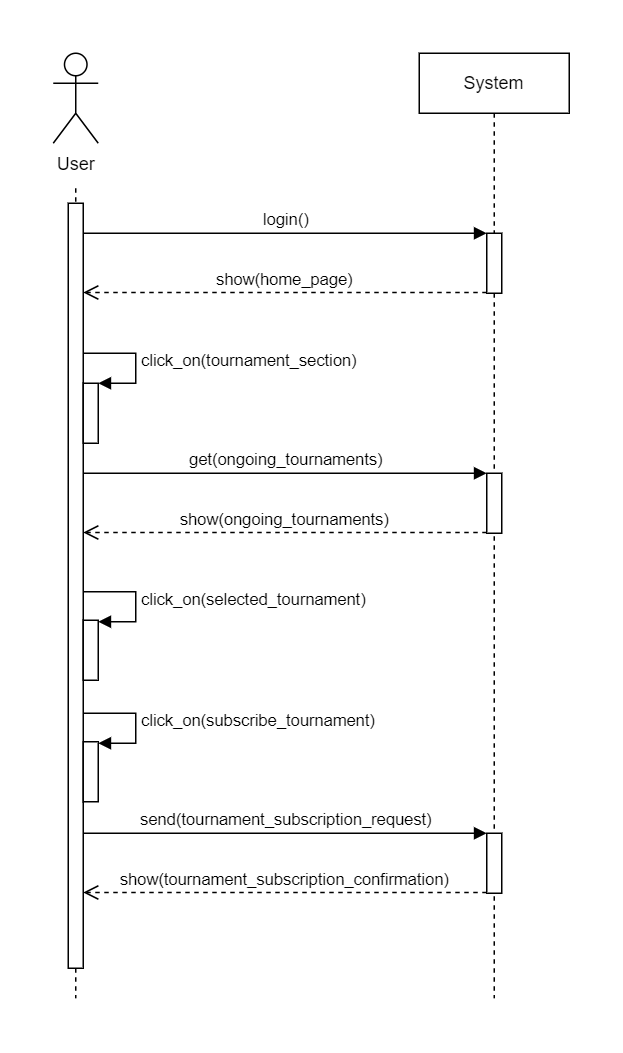
\includegraphics[width=0.73\textwidth]{../assets/section_3/SubscribeToATournament.png}
    \end{figure}
    \newpage

    \newgeometry{top=3em}
    \textbf{Create a group}
    \begin{figure}[h!]
        \centering
        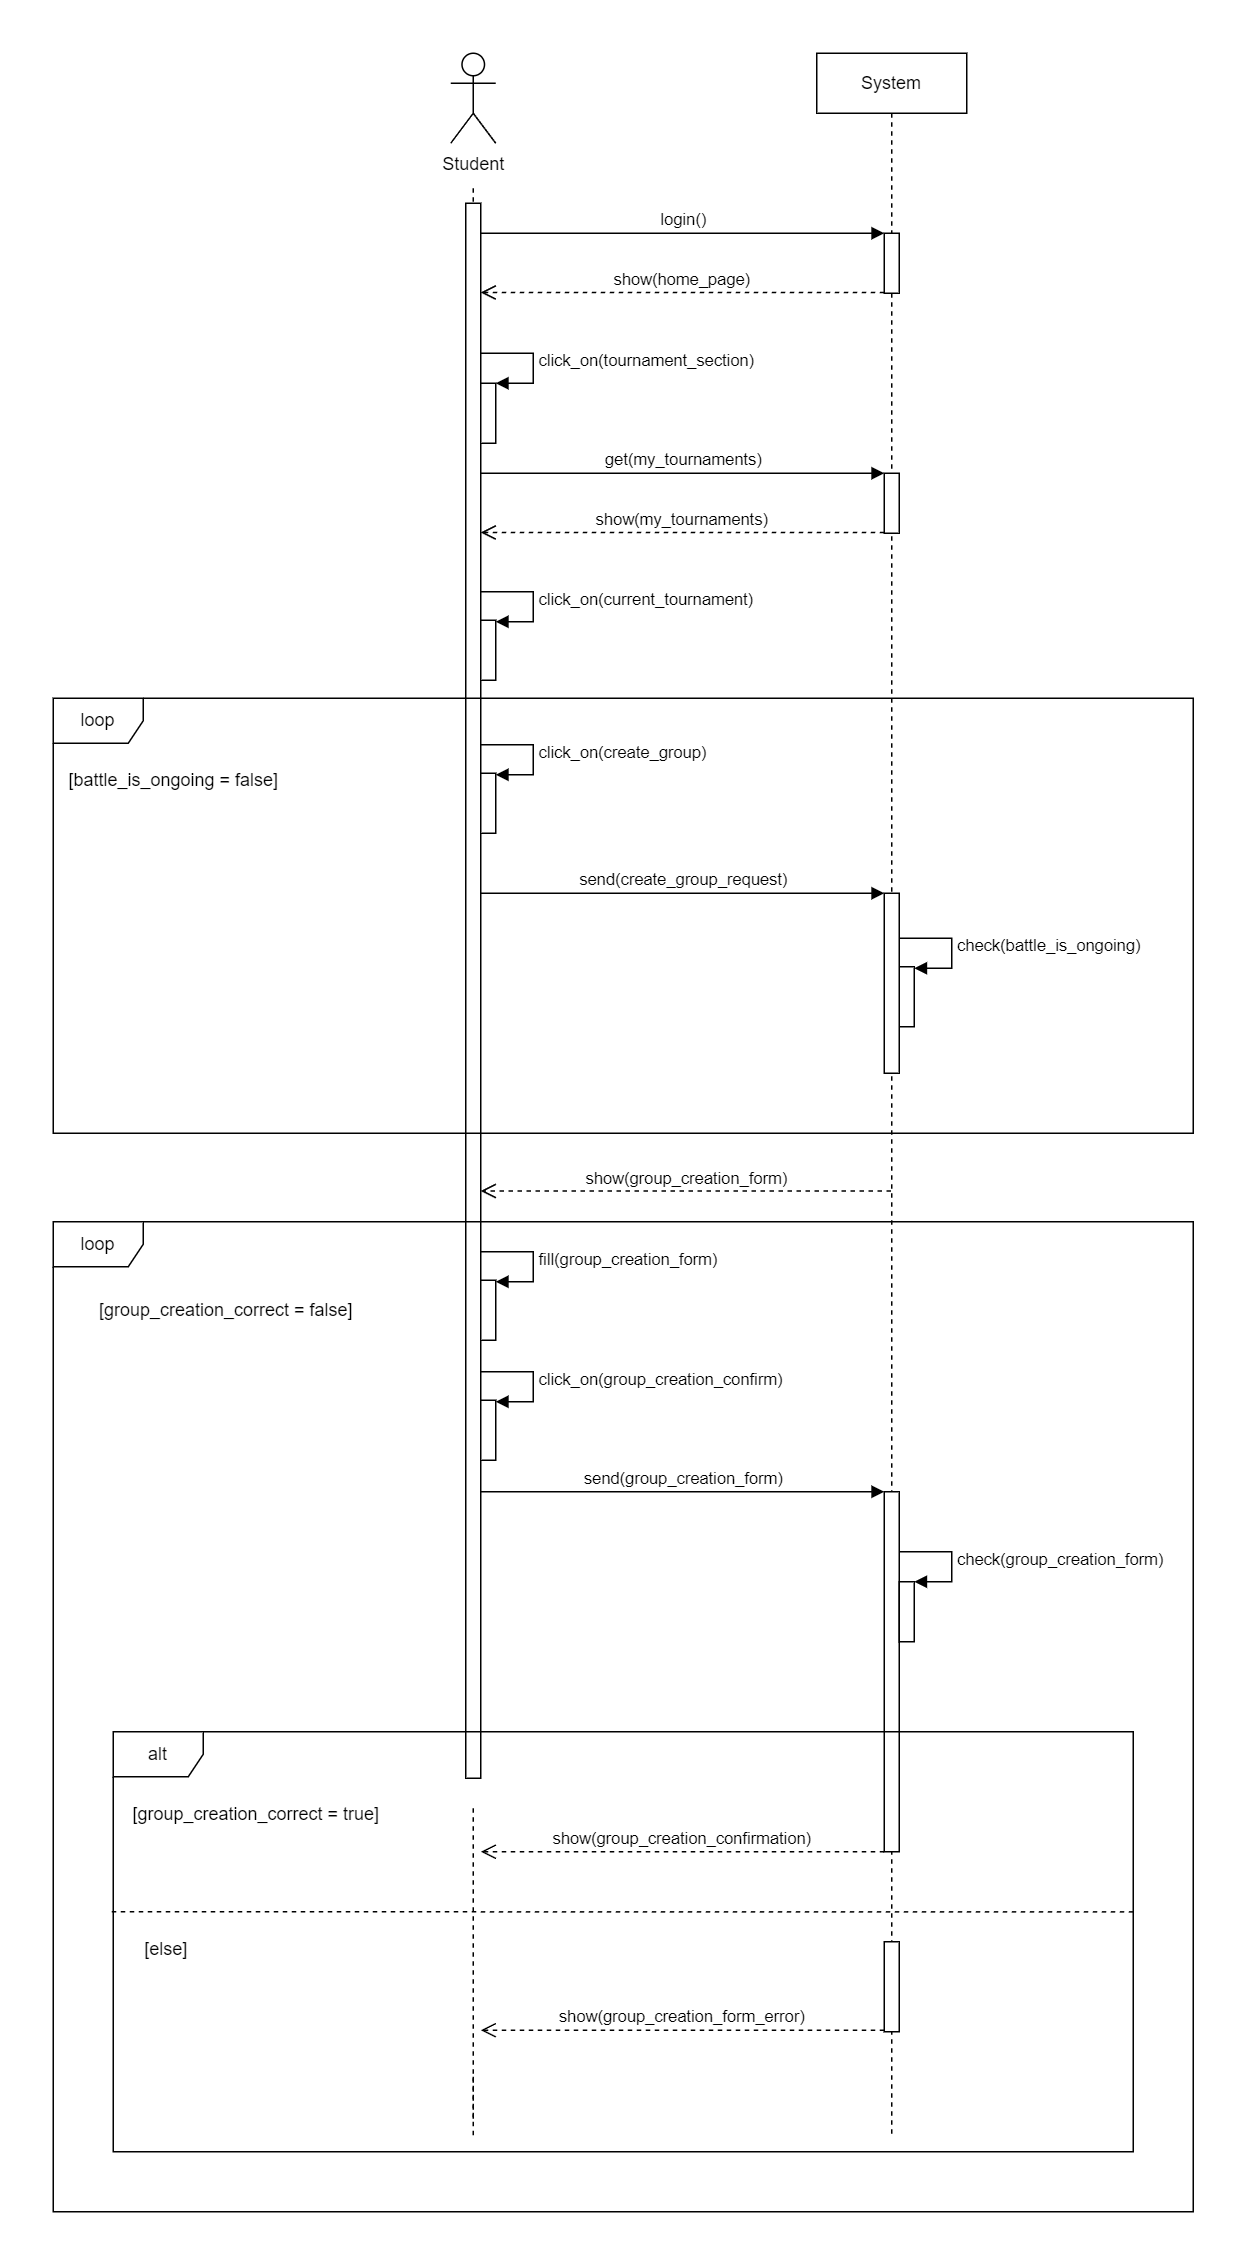
\includegraphics[width=0.8\textwidth]{../assets/section_3/CreateAGroup.png}
    \end{figure}
    \newpage
    \restoregeometry

    \newgeometry{top=8em}
    \textbf{Enroll in a battle}
    \begin{figure}[h!]
        \centering
        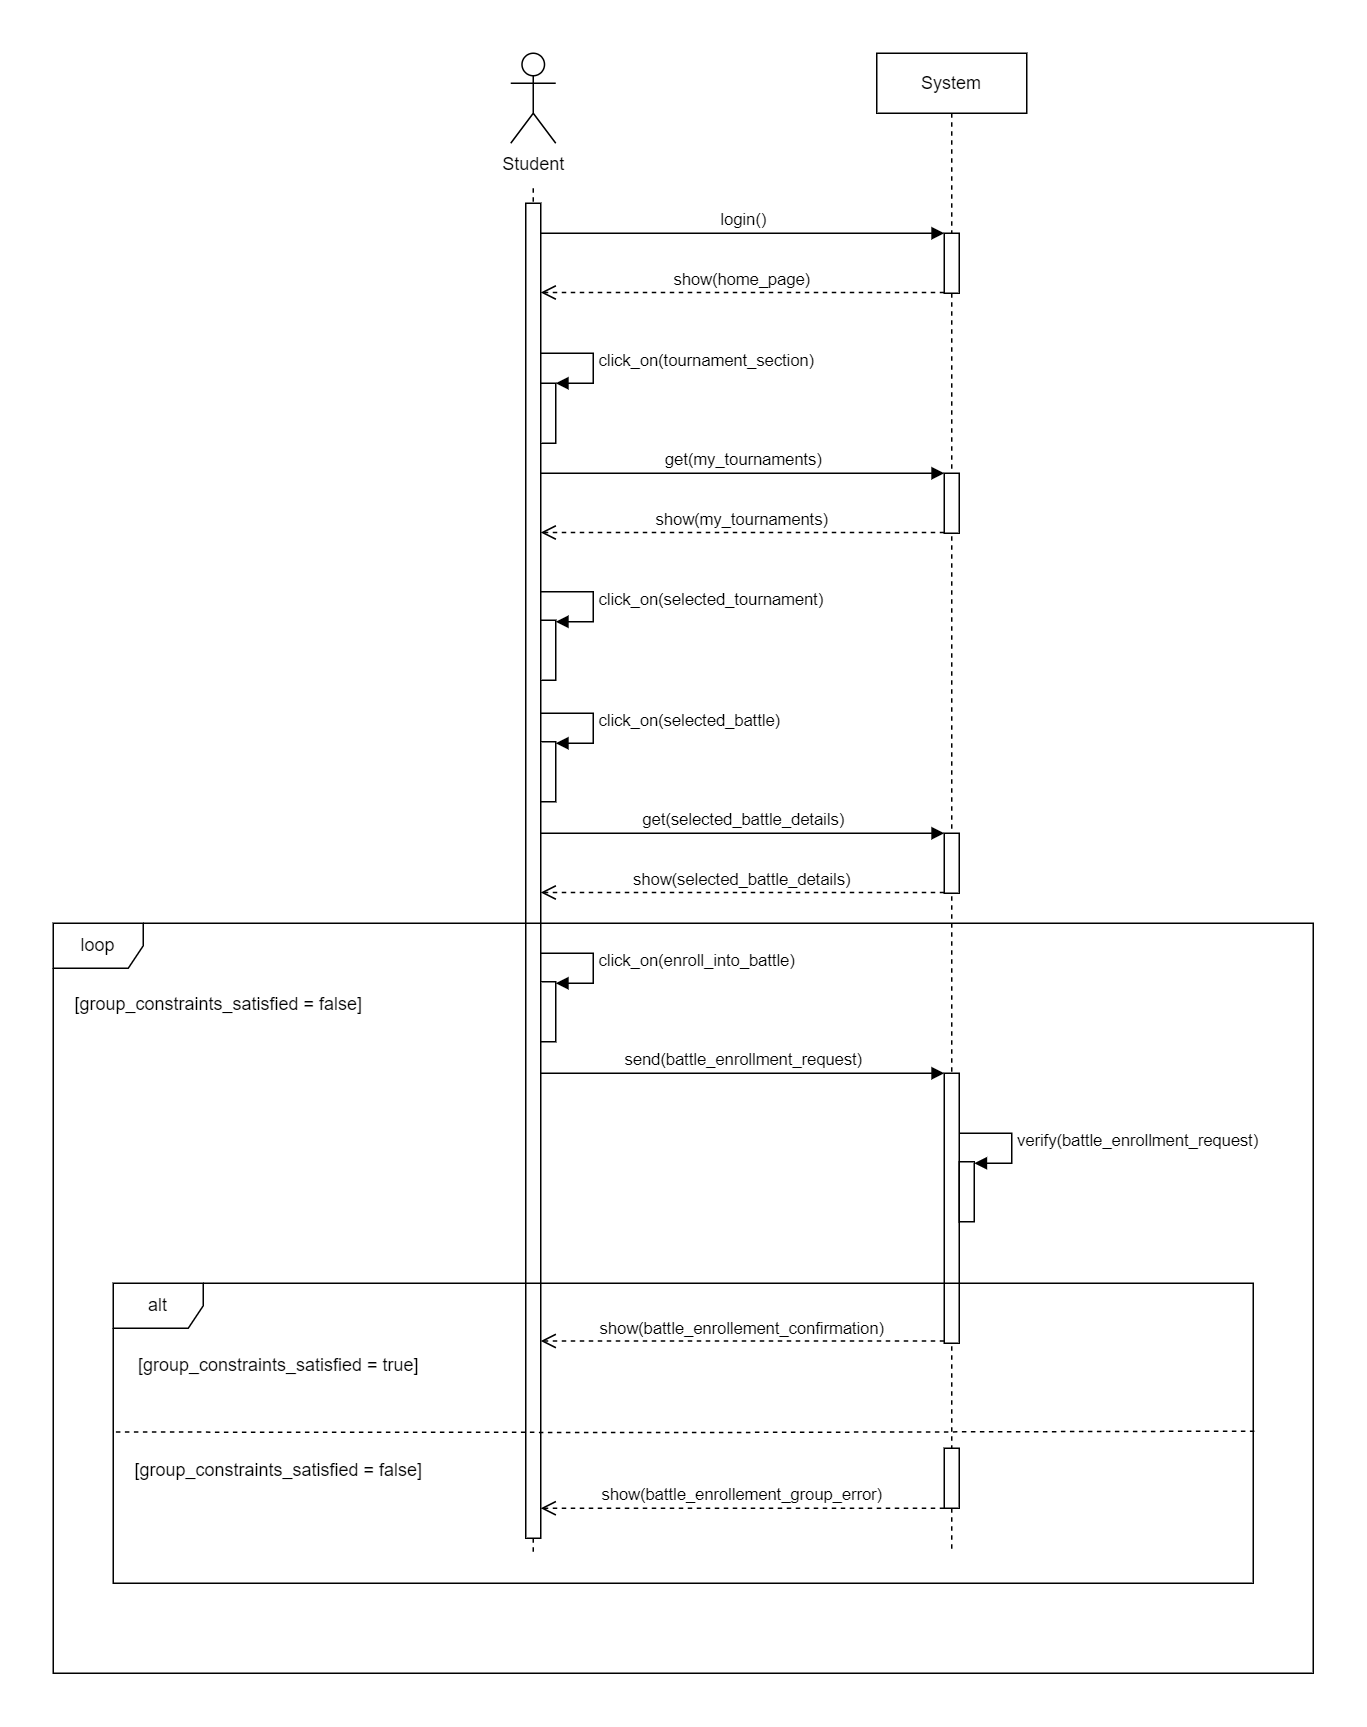
\includegraphics[width=1\textwidth]{../assets/section_3/EnrollInABattle.png}
    \end{figure}
    \newpage
    \restoregeometry

    \newgeometry{top=8em}
    \textbf{Invite a student to an existing group}
    \begin{figure}[h!]
        \centering
        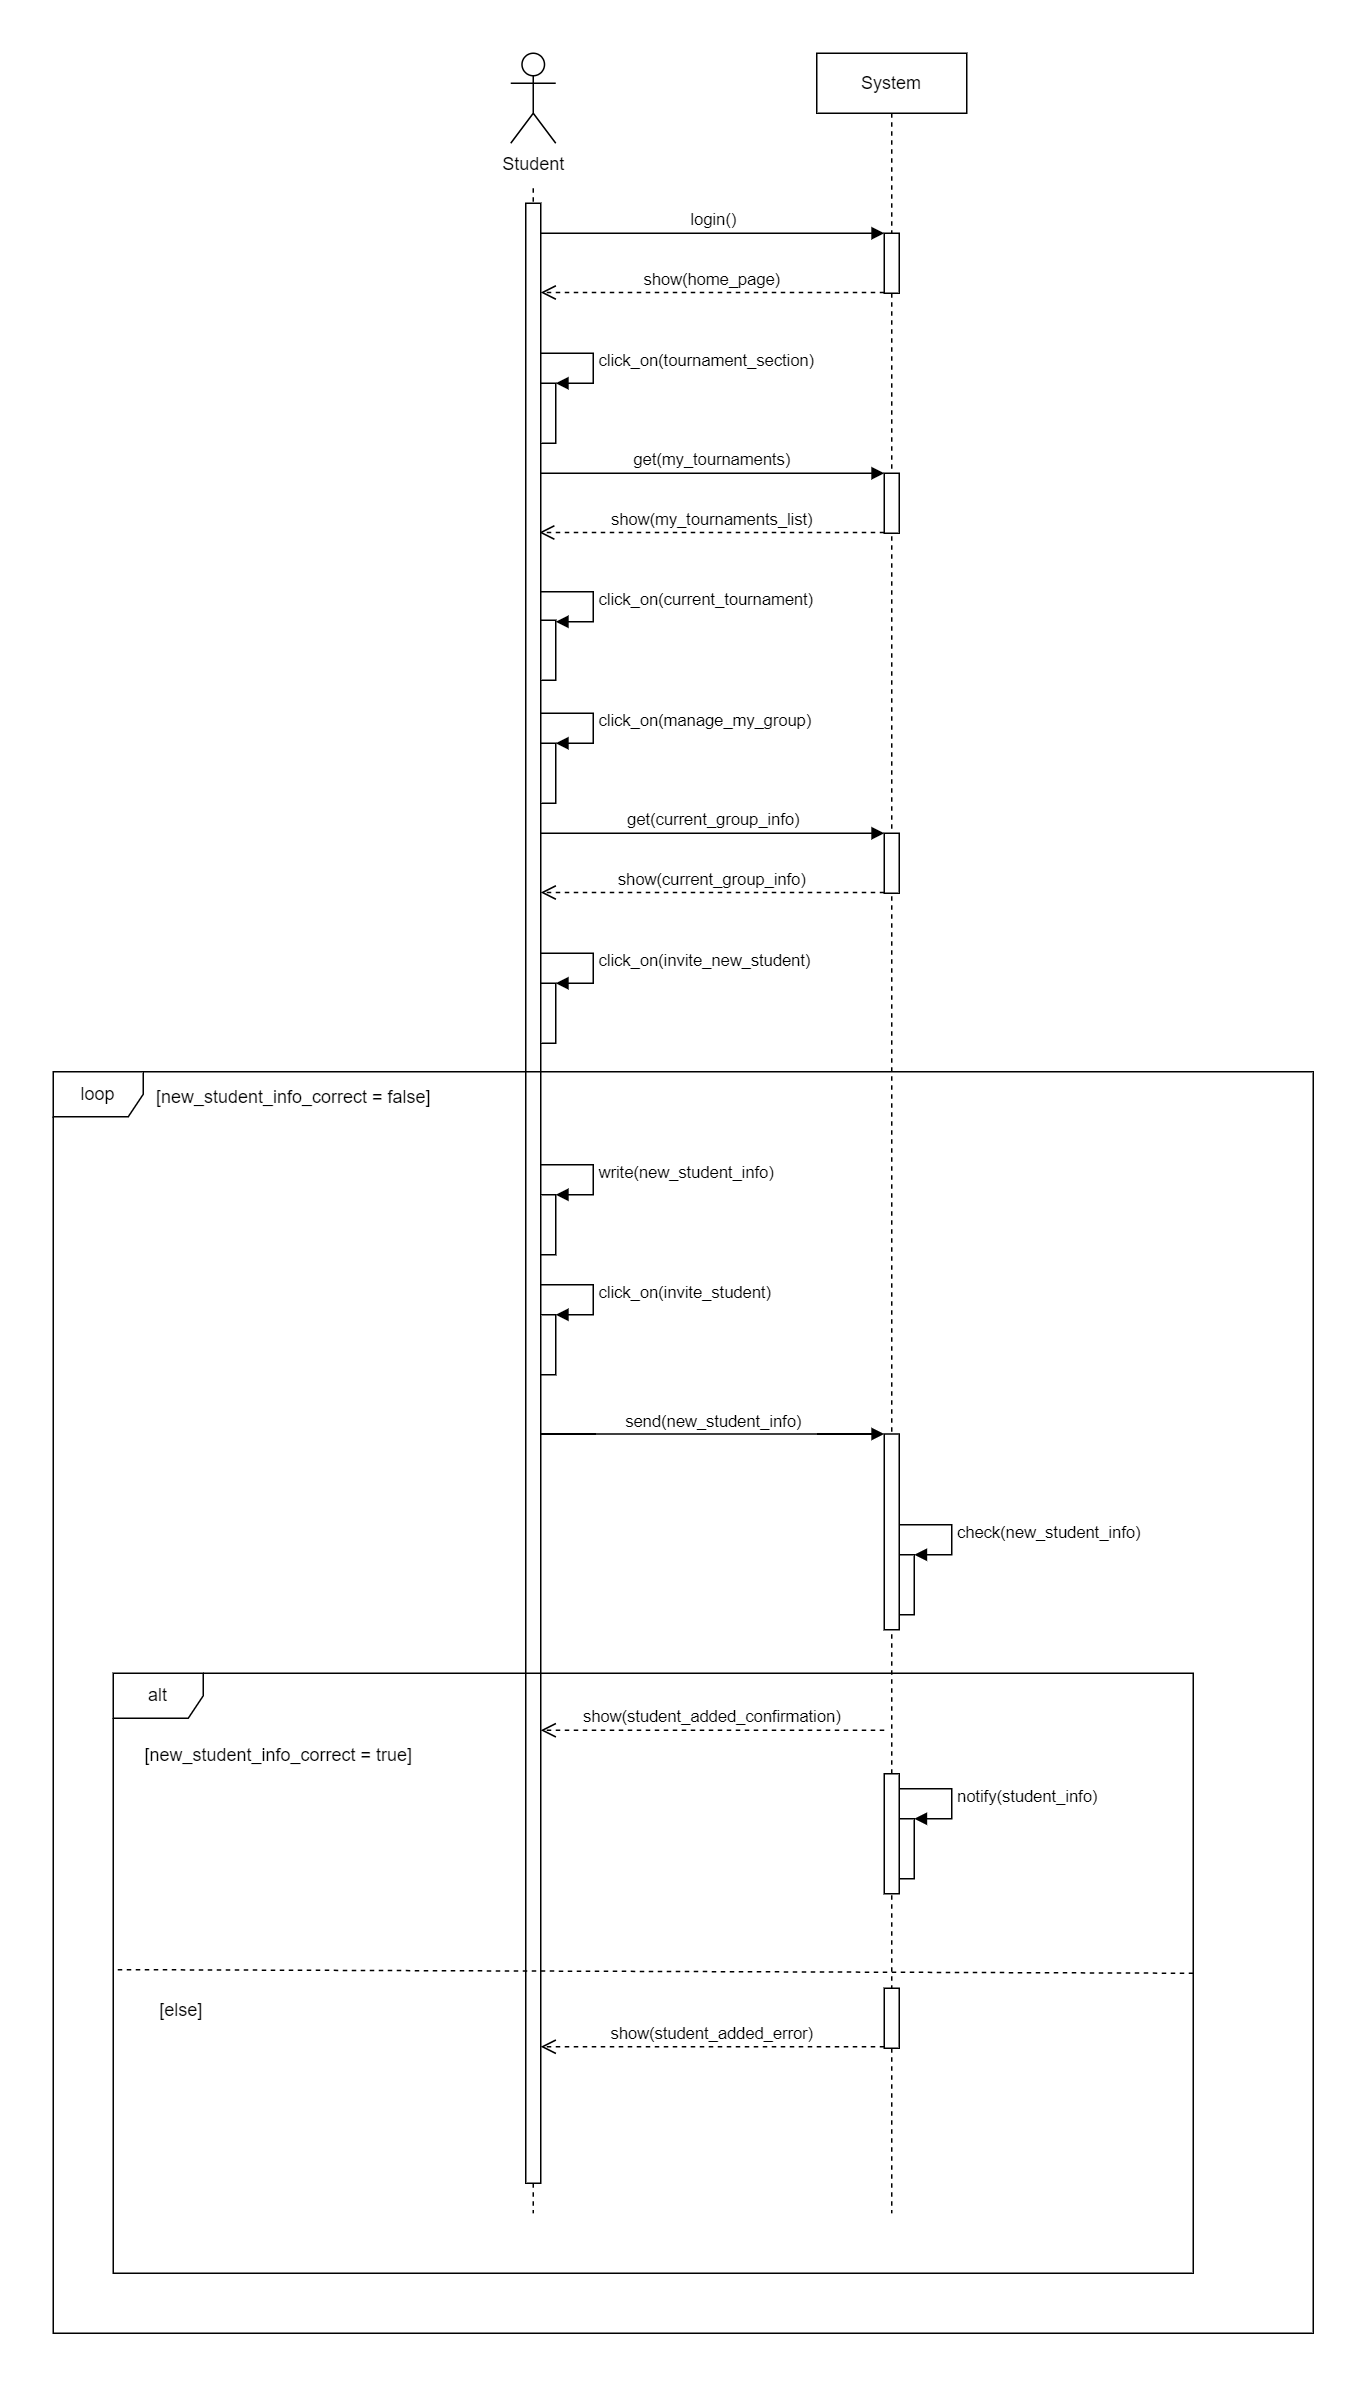
\includegraphics[width=0.75\textwidth]{../assets/section_3/InviteAStudentToAnExistingGroup.png}
    \end{figure}
    \newpage
    \restoregeometry

    \textbf{Student delivers a solution}
    \begin{figure}[h!]
        \centering
        \hspace*{2cm}
        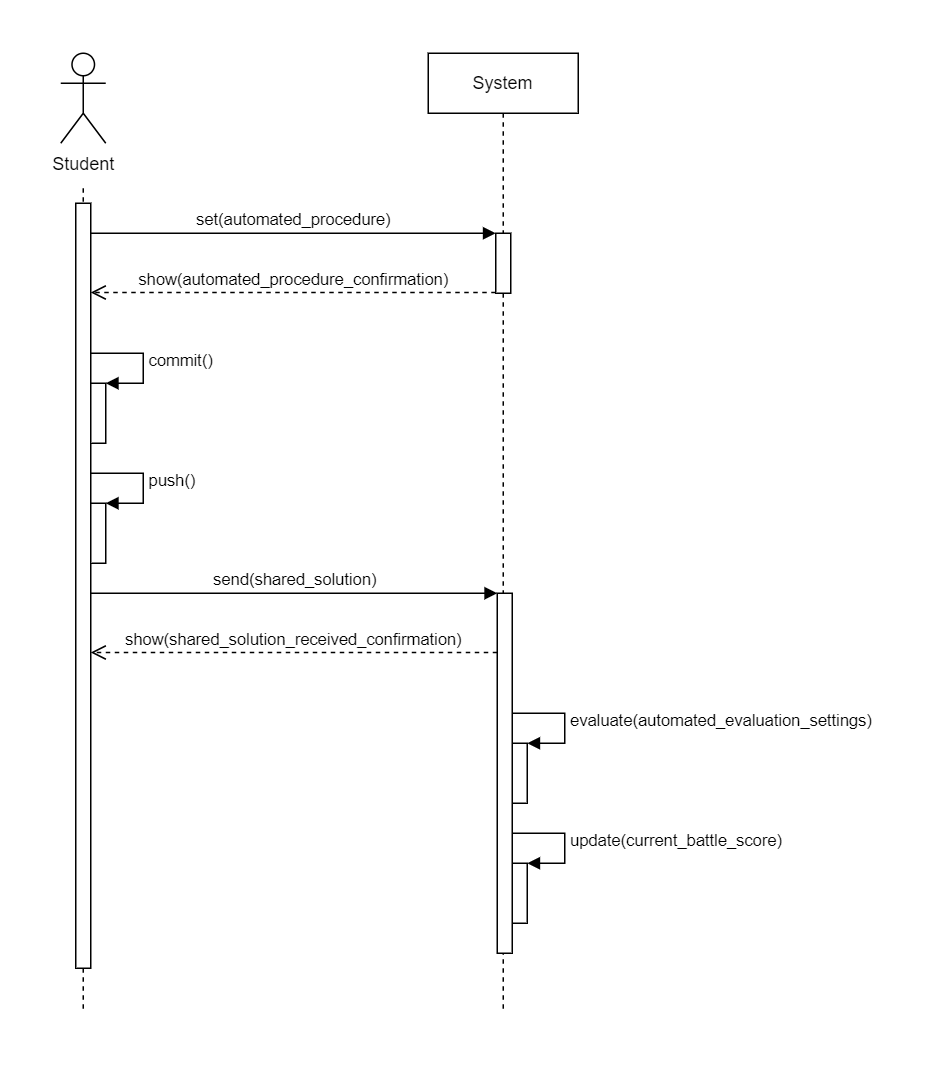
\includegraphics[width=1\textwidth]{../assets/section_3/GroupStudentDeliversASolution.png}
        \hspace*{-2cm}
    \end{figure}
    \newpage

    \textbf{Educator does a manual code review}
    \begin{figure}[h!]
        \centering
        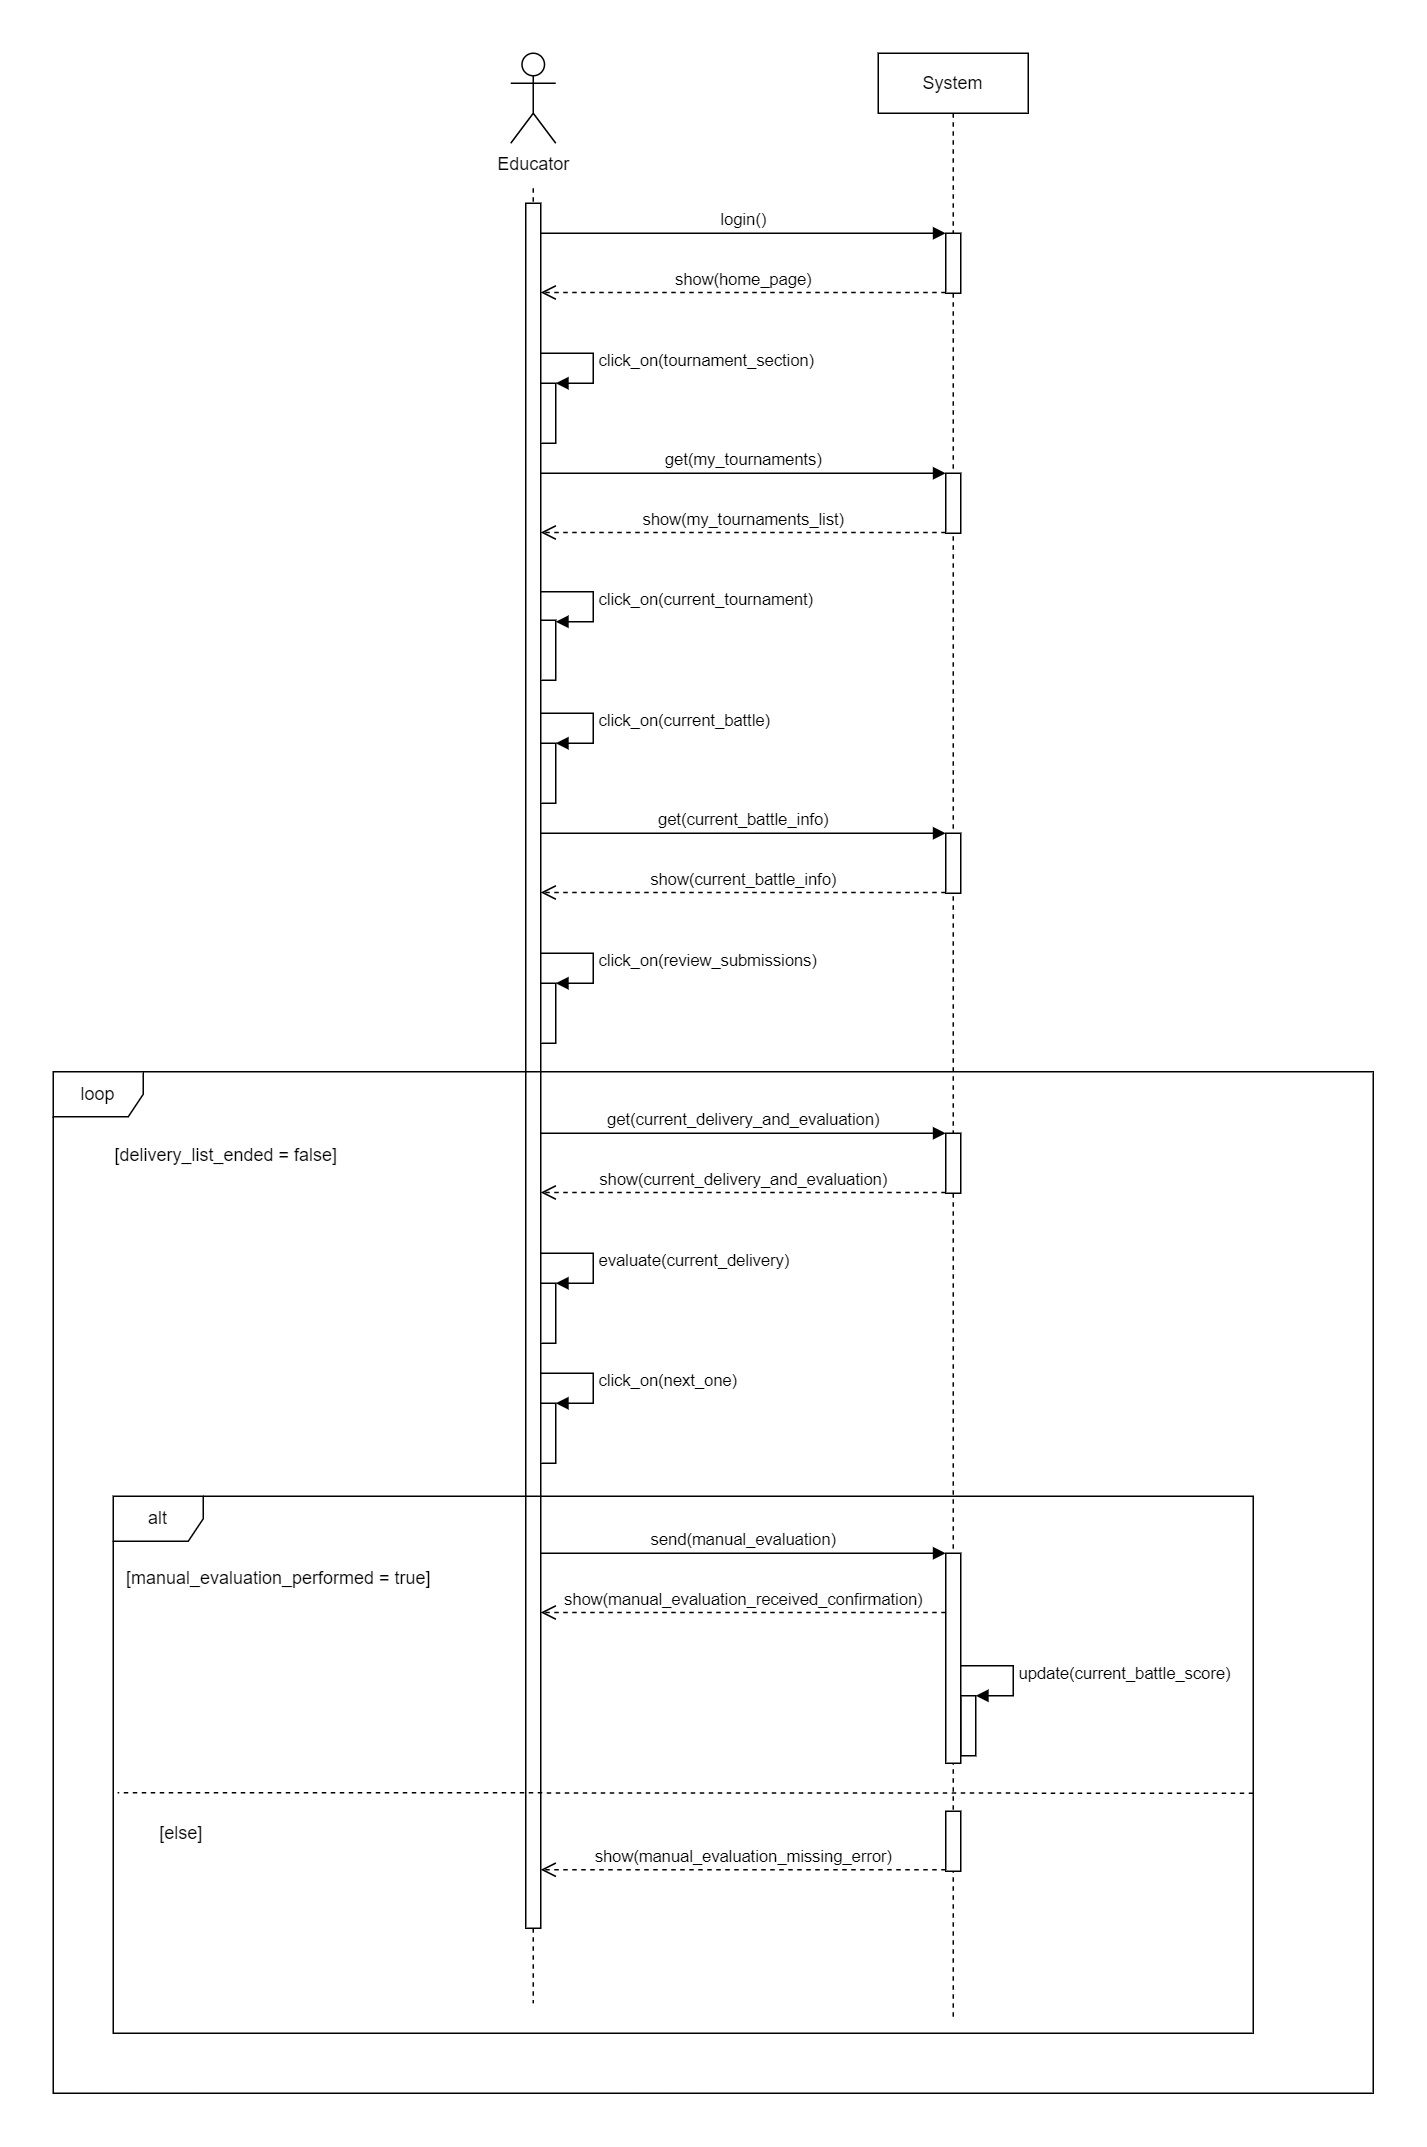
\includegraphics[width=0.8\textwidth]{../assets/section_3/EducatorDoesAManualCodeReview.png}
    \end{figure}
    \newpage

    \newgeometry{top=8em}
    \textbf{Close a battle early}
    \begin{figure}[h!]
        \centering
        \hspace*{1cm}
        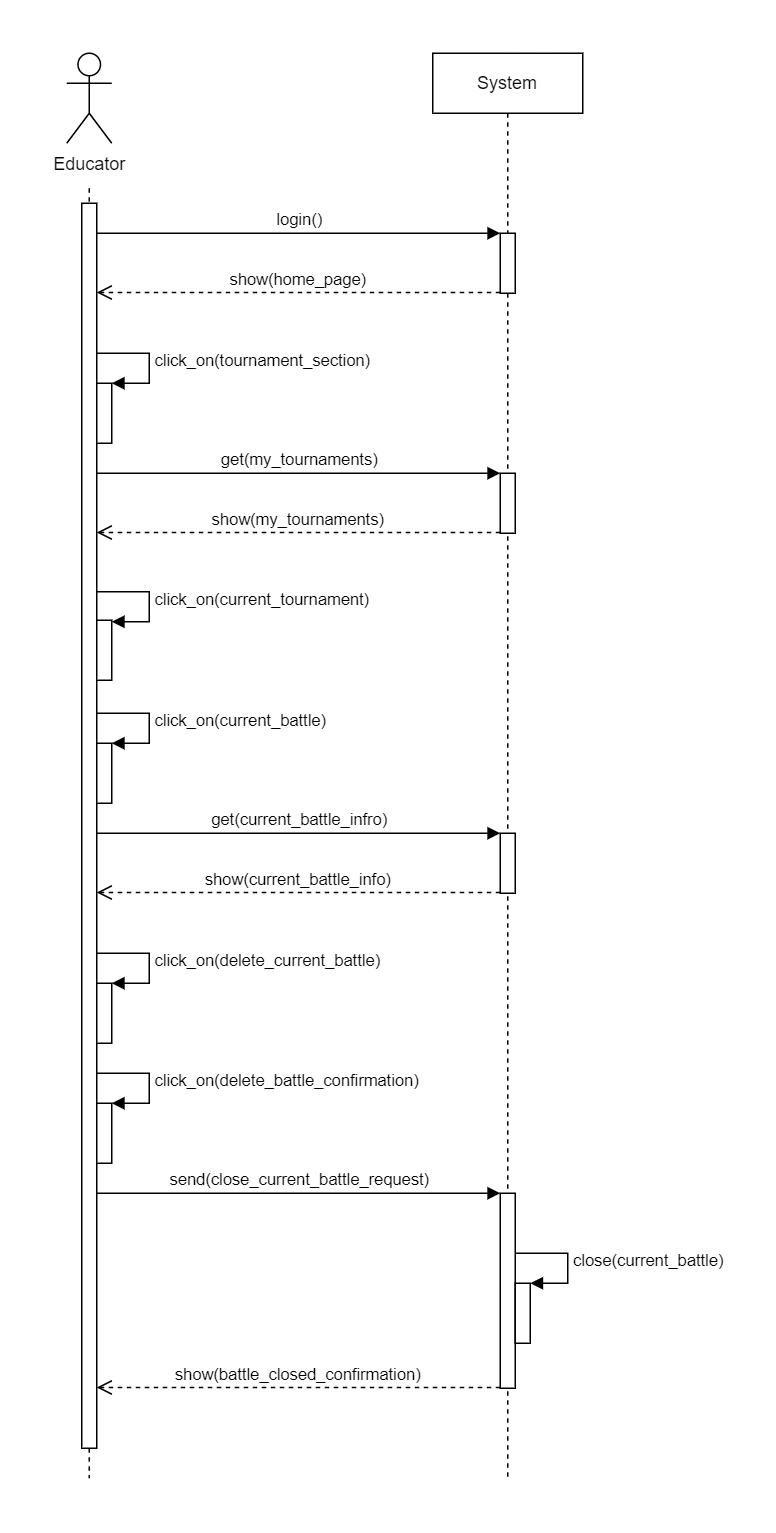
\includegraphics[width=0.65\textwidth]{../assets/section_3/CloseABattleEarly.png}
        \hspace*{-1cm}
    \end{figure}
    \newpage
    \restoregeometry

    \newgeometry{top=8em}
    \textbf{Close a tournament}
    \begin{figure}[h!]
        \centering
        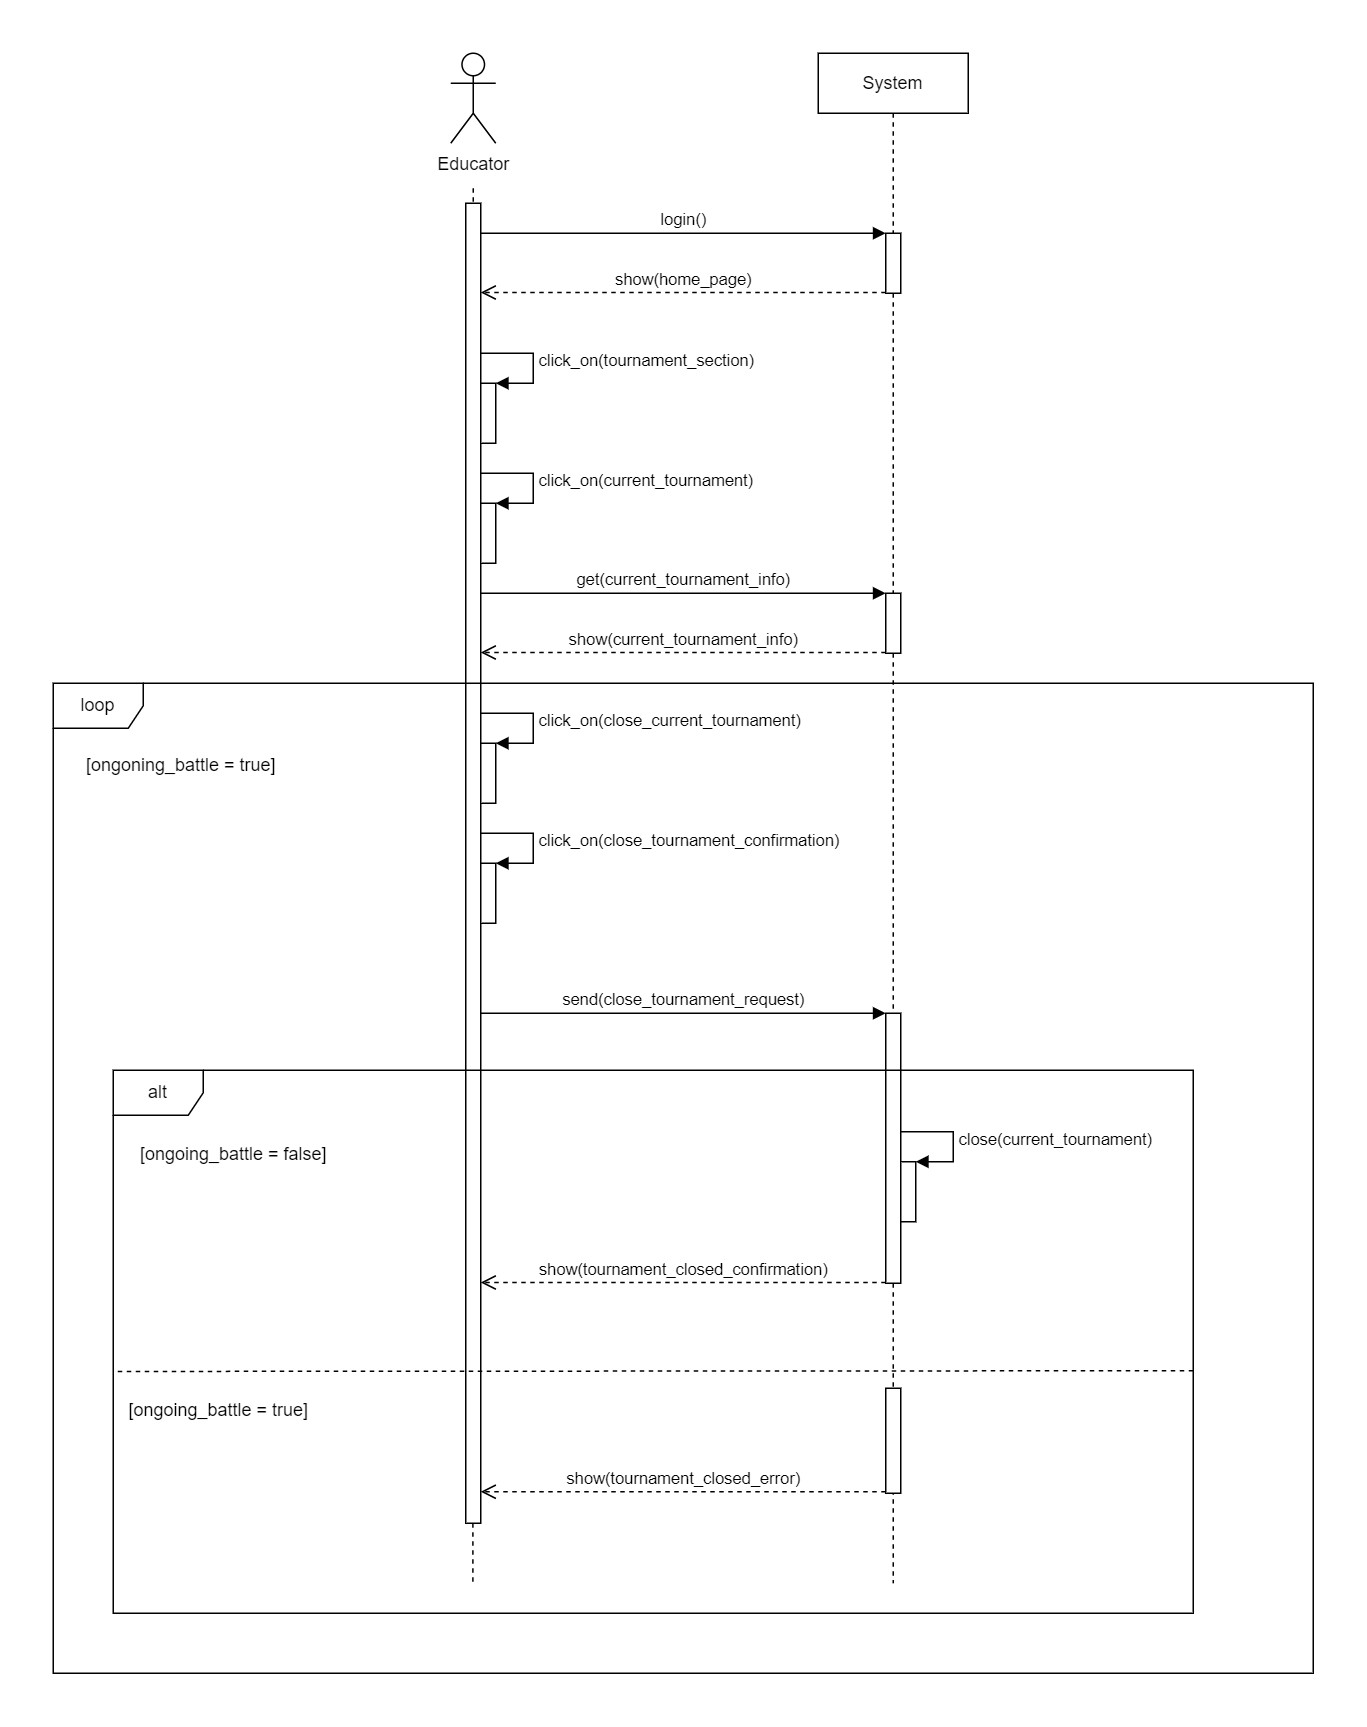
\includegraphics[width=1\textwidth]{../assets/section_3/CloseATournamentEarly.png}
    \end{figure}
    \newpage
    \restoregeometry

    \subsection{Performance Requirements}
        Given the fact that in each of our battles it will be mandatory for the system to evaluate the timeliness of the delivery, it is of paramount importance for us to guarantee that as less time as possible is lost on our side to evaluate the solutions and to send back our results, (consisting in the new student's rank and battle score) to give each student participating in the battle as much time as possible to fix his/her mistakes and eventually submit a new solution. Unfortunately, we cannot interfere with each student's own transmission speed, so we'll only need to focus on how our system will behave once that new delivery becomes readable, while keeping also in mind that faster equipment will also be more expensive, so we have to balance those two contrasting needs.\\
        Therefore, we should be able to check whether a new solution has been delivered at least once every second, and have a fast computational speed to be able to evaluate a solution of average length, in a situation of average workload in at most 3 seconds.\\
        Finally, estimating the number of concurrent active user that we should expect is a hard question, since we have very few data regarding this topic, but we can see that a website with a similar structure called \url{www.codewars.com} has on average 2.4M access each month\cite{CodeWars data}, so we can assume for it to have an average of 833 concurrent user active at the same time\footnote{to calculate this approximate value we have assumed the user session on our website to last on average 15 minutes and the access to be uniformly spread over the course of the whole day and month, therefore we have assumed that every access made in the same quarter of hour will be considered concurrent: $\text{concurrent\_acceses} = \frac{\text{monthly\_acces}}{30*24*4}$}, therefore given the minor popularity that our system will have initially but also to deal with peak hours the system is required to be able to handle up to 1300 concurrent active users\newpage

    \subsection{Design Constraints}
        \subsubsection{Standards compliance}    
            CodeKataBattle's user data must be compliant with the European Union's General Data Protection Regulation (GDPR), a European Union regulation on information privacy, therefore the system must be able to store and process user data securely, and must be able to provide the user with a way to access, modify or delete his/her own data at any time.
    
        \subsubsection{Hardware limitations}
            Given the nature of the software, not much computational power is needed on the user-side, so any fairly powered machine would probably be enough for our users to effectively use the software. On the other hand an internet connection is required, in order to communicate and exchange data with the platform, and this internet connection is also strongly suggested to be fast and stable in order to grant the user a fair competition with his/her opponents (for example to avoid delays while reading the code kata, sending the delivery or receiving his/her updated battle score)

    \subsection{Software System Attributes}
        \subsubsection{Reliability}
            The system must have a backup infrastructure to ensure that the data is always available and that the system can be restored in case of a failure. The components of this infrastructure must be characterized by a high MTTF (Mean Time To Failure) and a low MTTR (Mean Time To Repair), in order to both reduce the amount of failures to a minimum and to be able to quickly recover when those failures actually happen. Moreover, all the needed components must be redundant and parallelized as much as possible, to ensure a high reliability of the overall system as well as fault-resilience in the case of a single component failure\newpage
        
        \subsubsection{Availability}
            CodeKataBattle is not an emergency service or anything related to critical situations, so it is considered enough for the system to provide an availability of 99.9\%, this means an average downtime of 8.77 hours per year, or 10.08 minutes a week, which is perfectly fine for our uses.\\
            Also, since CKB is expected to be used also by teacher during exercise classes and by student/workers in days when they are not going to school or work, the peak hours are expected to be from 9 to 12 during working days and from 15 to 19 during weekends, so the system should be able to handle a higher than average workload during these time-slots. For this reason all the maintenance activities should be done at night from Monday to Thursday when the system is less used.    

        \subsubsection{Security}
            The system store some sensitive personal information about its users, so the security aspect cannot be under-estimated, the data stored by the system must be protected and its communication with other components must be encrypted, to avoid any unauthorized interception.\\
            Therefore, all the user data must be stored securely, hashed and/or encrypted using approved algorithms that have not been cryptographically broken, like SHA-256 for hashing or AES-256 for encryption. Specifically, passwords should be stored only in their hashed version and subsequently the whole data stored regarding a user (including the hashed password) should be encrypted.\\  Furthermore, the communications between the server and any other component or external entity should be encrypted using TLS 1.3 and powered by HTTPS, to grant confidentiality, integrity, and authenticity to such communications.\\
            Finally, all stored data must be compliant with the GDPR.\newpage

        \subsubsection{Maintainability}
            The system must be easy to maintain and update, and must be able to be extended with new features in the future with ease. For this reason the system must be designed using a modular architecture, and must be developed using modern design patterns and best practices guaranteeing high reusability of its code, as well as future extensions of its features. A documentation for such code must also be produced which should be clear, complete and easy to understand. Finally, the system should also be tested using unit tests and integration tests covering all its modules before its release, to assert that no errors or conflicts are present       

        \subsubsection{Portability}
        The system should be designed to be easily ported into many platforms, providing equal functionalities in each of these versions, for example the system could be designed to work with most modern web browsers (like Google Chrome,  Microsoft Edge, Mozilla Firefox, Opera or Safari, as well as possibly other Chromium based web browsers) and/or most of the modern desktop and mobile operating systems (like Windows, macOS, Linux, Android or iOS).

\end{document}